\RequirePackage{float} % Need to load the float package before hyperref, so hyperref detects and patches it, so when we load minted later it uses the patched \newfloat (minted loads float). More info here: http://tex.stackexchange.com/questions/19371/minteds-listing-environment-with-hyperref-and-caption-package-together
\documentclass[twoside,english,a4paper]{uiofysmaster}
\usepackage{lmodern}
\usepackage[T1]{fontenc}
\usepackage[utf8]{inputenc}
% \usepackage[top=1.5in, bottom=1.5in, left=1in, right=1in]{geometry} % Correct geometry in uiofysmaster

% ----  biblatex ---- %
\usepackage[english]{babel}
\usepackage{csquotes}
\usepackage[backend=biber, sorting=none]{biblatex} % Note that "sorting=none" is NOT the same as leaving the field blank, "sorting=none" means "sorting=citeorder".
\bibliography{JabRef_database,Mendeley_database}

% ---- Code syntax highlighting ---- %
\usepackage[scaled=0.8]{beramono}  % Better monospaced font, nice ~ and ^
% \usepackage[chapter]{minted} % included in uiofysmaster package, to load it before hyperref, to fix \listoflistings
\definecolor{codebg}{rgb}{0.95,0.95,0.95}
\newminted[cppcode]{cpp}{ % can use \newminted{cpp}, gives the same result
    mathescape,
%     frame=lines,
%     framesep=2mm,
    bgcolor = codebg,
    fontsize = \small,
%     fontfamily = courier
} 
% usage: \begin{cppcode}
% use \begin{cppcode*}{<extra options>} if you want to add extra options on the fly

% More options:
% \renewcommand\listingscaption{Program code}
% \renewcommand\listoflistingscaption{List of program codes}

% ----  Draft stuff (remove before final version) ---- %
\usepackage{todonotes}
\usepackage{xcolor}
\newcommand{\orangebox}[1]{
    \fcolorbox{black}{orange}{
        \begin{minipage}{\textwidth}
            #1
        \end{minipage}
    }
}
\usepackage{soulutf8}       % To highlight stuff (when using utf8), using \hl{}. Also has \st{} for strikethrough. Doesn't work that well with equations...
\usepackage{lipsum}

% ---- Images ---- %
\usepackage{graphicx}
\usepackage{svg}            % To include .svg vector graphics directly using \includesvg (will automatically compile/convert the images to .pdf+.pdf_tex using Inkscape). 
                            % NEEDS ``pdflatex --shell-escape'' !!!
\setsvg{                    % conversion options for svg package
    inkscape = inkscape -z -D
}
\usepackage{subcaption}     % The subfigure and subfig packages are deprecated and shouldn't be used any more: 
                            % http://tex.stackexchange.com/questions/144782/subfigure-and-subfig-packages-deprecated
                            % the svg-package originally uses subfig, but replacing subfig with subcaption seems to work
% ---- Other stuff ---- %
% \usepackage{minipage}
\usepackage{commath}        % To correctly typeset differentials \od[2]{f}{x}, \dod, and \tod
\usepackage{fancyvrb}       % Better verbatim, that works inside fcolorbox. Usage: \begin{Verbatim} or \Verb!verbatimThing!
\usepackage{cleveref}       % NEEDS TO BE LOADED AFTER hyperref? (at least something in preamble/preamble.tex) Use \cref{fig:label} instead of \ref{} to get auto ``fig. 1.1a''. \Cref for capitalized.
\usepackage{upgreek}        % Upper case greek letters
\usepackage{bm}             % Bold symbols in math mode
\usepackage{mathtools}      % Mainly for \vdotswithin{=} and \shortvdotswithin{=}
\usepackage{pdfpages}       % To include the frontpage pdf
% \usepackage{hyperref}       % Load hyperref package last % Loaded by uiofysmaster
% \usepackage{paralist}
\usepackage{relsize}        % To resize stuff - specifically integration signs
\usepackage{exscale}        % To resize integration sign twice, ``\DeclareMathOperator{\biggerint}{\mathlarger{\mathlarger{\int}}}''
\usepackage{braket}         % Dirac bra/kets, \Bra{a}, \Ket{b}, \Braket{a|b|a}. \Braket auto stretches \l/rangles and |'s
% \usepackage{float}        % Put at top of master using \RequirePackage{float}, to fix minted/hyperref/float
\usepackage{placeins}       % Stop floats from going past somewhere by adding \FloatBarrier. This makes all floats before the barrier appear before the barrier in the pdf

% ---- Custom itemize ---- %
\usepackage{enumitem}       % Better control over enu­mer­ate, item­ize and de­scrip­tion. Su­per­sedes both enu­mer­ate and md­wlist.
\SetEnumitemKey{midsep}{topsep=3pt,partopsep=3pt,parsep=3pt,itemsep=3pt}

% ---- Custom lengths for figures ---- %
% (so we can just use \setlength later)
\newlength{\myfigwidth}
\newlength{\mycaptionwidth}

% ---- Custom commands and symbols ---- %
% ----- Vectors ---- %
% \newcommand{\bvec}[1]{\mathbf{#1}}
\newcommand{\oldvec}{\vec}
\newcommand{\bvec}[1]{\boldsymbol{#1}}      % Using amsmath's boldsymbol
\renewcommand{\vec}{\bvec}
% \newcommand{\bvec}[1]{\bm{#1}}
\newcommand{\rvec}{\bvec{r}}
\newcommand{\vvec}{\bvec{v}}
\newcommand{\avec}{\bvec{a}}
\newcommand{\Fvec}{\bvec{F}}
% ---- Other math commands and symbols ---- %
% \newcommand\diff{\mathop{}\!\mathrm{d}}   % Already defined as \dif by commath! But maybe this way is better? Commath uses ``\DeclareMathOperator{\dif}{d \!}''
\DeclareMathOperator{\diff}{d \!}           % See top comment on this reply: http://tex.stackexchange.com/a/95681/31078
% \newcommand\Ham{\mathop{}\!\mathrm{\mathcal{H}}}
\DeclareMathOperator{\Ham}{\mathcal{H}}
% \newcommand\bigint{\mathop{\mathlarger{\int}}}
\DeclareMathOperator{\bigint}{\mathlarger{\int}}
% \newcommand\deltaop{\mathop{\!\mathrm{\delta}}}
% \DeclareMathOperator{\deltaop}{\updelta \!}
\DeclareMathOperator{\deltaop}{\updelta}
% \newcommand\biggerint{\mathop{\mathlarger{\mathlarger{\int}}}}
\DeclareMathOperator{\biggerint}{\mathlarger{\mathlarger{\int}}}
% ---- Other ---- %
\newcommand{\Ang}{\AA ngstr\"om}
\newcommand{\Schr}{Schr\"odinger}

% ---- Fix unicode stuff ---- %
\DeclareUnicodeCharacter{2212}{-}   % Unicode 'MINUS SIGN' (U+2212) that matplotlib uses for minus on axis tick labes

% ---- Formatting ---- %
% skip line instead of indent on new paragraph
\setlength{\parskip}{11pt}
\setlength{\parindent}{0mm}
% make figure text more narrow than textwidth, use small font, and make ``figure'' bold
% ! see alternatives in FYS4180 report
\captionsetup{width=.9\textwidth}
\captionsetup{font=small,labelfont=bf}

\author{Filip Sund}
\title{\uppercase{Water confined in nanoporous media}}
\date{June 2014}

% \includeonly{molecular_dynamics/simulations}
% \includeonly{fractures/fractures}
\begin{document}

\pagenumbering{roman}

\includepdf{frontpage.pdf}
\cleardoublepage

\begin{abstract}
\todoa{Check distance before and after \AA and \cpp and similar commands}
    \lipsum[1-4]
\end{abstract}
\begin{dedication}
  To someone
  \\\vspace{12pt}
  \lipsum[1-4]
\end{dedication}
\begin{acknowledgements}
``This work was performed on the Abel Cluster, owned by the University of Oslo and the Norwegian metacenter for High Performance Computing (NOTUR), and operated by the Department for Research Computing at USIT, the University of Oslo IT-department. \url{http://www.hpc.uio.no/}'' \todo{most were done on smaug though}

Thanks to Ovito\cite{stukowski2010ovito} and Inkscape\cite{webinkscape}

\end{acknowledgements}


\tableofcontents

\listoffigures
\listoftables
\listoflistings

\chapter*{Introduction}
\todoa{Cite Inkscape, Ovito}
\begin{itemize}
    \item Water confined in nanoporous silica
    \item Characterization of porous silica
    \item 
\end{itemize}

\begin{center}
\begin{table}
    \begin{tabular}{ | l | l | l | p{5cm} |}
    \hline
    Day & Min Temp & Max Temp & Summary \\ \hline
    Monday & 11C & 22C & A clear day with lots of sunshine.  
    However, the strong breeze will bring down the temperatures. \\ \hline
    Tuesday & 9C & 19C & Cloudy with rain, across many northern regions. Clear spells
    across most of Scotland and Northern Ireland,
    but rain reaching the far northwest. \\ \hline
    Wednesday & 10C & 21C & Rain will still linger for the morning.
    Conditions will improve by early afternoon and continue
    throughout the evening. \\
    \hline
    \end{tabular}
\caption{A table for the list of tables, so it won't become envious of the other lists.}
\end{table}
\end{center}


\part{Molecular dynamics}
    \chapter{Introduction}
{\fontfamily{fdm}\selectfont test}
\mono{test2}

In this chapter we will give an overview of how simulations of atomic systems are done using molecular dynamics. We will show the theory that makes molecular dynamics so efficient and useful, and we will show how to build up and implement a molecular dynamics program. The program used for producing the results presented in this thesis uses a much more sophisticated model for the interactions between the atoms, and is parallellized and highly optimized for doing calculations on high-performance computing clusters like Abel. We will nevertheless gain a lot of insight into this program by starting with a a simpler case.

% To accurately study molecular many-body systems like water confined in nanoporous silica means that we have to consider the quantum mechanical nature of atoms and molecules. To study the motion of atoms using \hl{ab-initio} quantum mechanical calculations, where we have to consider the effect of all electrons, protons and neutrons for all atoms, we have to solve a problem with dimensionality 
% 
% To study water confined in nanoporous silica we use the the method of molecular dynamics simulations. This is a method that use knowledge from the complex quantum mechanical nature of atoms and molecules, to reduce the many-body problems  create simple potentials only depending on the positions \hl{(and velocities?)} of atoms represented as point particles, which we can integrate using Newton's equations of motion. 
% 
% to replacing heavy calculations on the wavefunctions of electrons, protons and neutrons with simple\hl{r} calculations only depending on the positions \hl{(and velocities?)} of point particles representing the positions of the atoms.
% 
% where we approximate the forces between atoms using potentials and parameters from studies and simulations of the underlying quantum mechanical nature of the atoms. This means that we don't have to calculate the exact quantum mechanical interactions between atoms, but instead model the atoms as point particles, with potentials depending on the positions \hl{(and velocities)} of the atoms that give rise to forces. By integrating the forces using Newton's equations of motion
% 
% To do an exact study of the behaviour of atoms and molecules we have to take into account the quantum mechanical workings of such a system. To a silica system we have to consider the that silicon and oxygen consist of  electrons, protons and neutrons of all atoms 

To do an exact study of a many-body atomic system like water confined in nanoporous silica, we have to take into account the quantum mechanical nature of the atoms and molecules in the system. An \hl{average} oxygen molecule consists of 8 electrons, 8 protons and 8 neutrons, all interacting with each other, and each with 3 translational degrees of freedom. This makes doing calculations on something as \hl{``simple''} an electron pretty complex if we want to do it properly. If we want to study a system consisting of more than a couple of oxygen atoms we see that the number of particles and degrees of freedom quickly makes the problem grow to intractable proportions. Since we are mainly interested in the equilibrium and transport properties of the system, we can reduce the problem to something we can handle by using results from underlying quantum mechanical calculations, to develop approximate models of the system. We assume that the many-body system behaves \hl{clasically}, and model all atoms as point particles. From quantum mechanical results we create potentials that approximate the exact forces between the atoms, that only depend on the position \hl{(and velocity?)} of the \hl{atoms/nuclei/point particles}, which are orders of magnitude faster to evaluate compared to calculating the exact forces between the atoms from quantum mechanical principles. We then solve Newton's equations of motion for the system.

To explain how a Molecular Dynamics simulation work we start with a simple example, using one atom type, and a simple model for the force between the atoms. This allows us to get an understanding of the basic concepts used in \hl{MD}. The program actually used for the calculations in the work presented in this thesis uses a very complex potential, and is highly optimized and parallellized for doing calculations on computing clusters on several hundred \hl{CPU's}. But the inner workings of that program \hl{is both a) too much to cover? and b) not necessary to explain?).}

    \chapter{Statistical mechanics}
% \hl{The idea behind Molecular Dynamics simulations is that we can study the average behaviour of a many-body system by computing the natural time evolution of the system numerically and averaging the quantity of interest over a sufficiently long time.} -- Frenkel p. 15
% 
% Before we start work on to do simulations using molecular dynamics, we need some basics on \emph{why} we can use MD to study atomic systems like silica and water. We first use the Born-Oppenheimer approximation to justify that the Hamiltonian of the system can be expressed as a function of the positions and velocities of the atoms, having averaged out the rapid motion of the individual subatomic particles (like electrons and protons). We then make the approximation that a classical description of the system is adequate, which we 
% 
% % To do this we need some \hl{something} from the field of statistical mechanics.
% 
% Using statistical mechanics stated in quantum mechanical terms, and using
% 
% The basic assumption behind statistical mechanics, from which much of statistical mechanics follows, is that a system with fixed number of particles $N$, volume $V$ and energy $E$ is equally likely to be found in any of its eigenstates. Using this assumption, and stating statistical mechanics in quantum mechanical terms, it can be shown that the probability for finding a system at temperature $T$ in quantum state $i$ is
% \begin{align}
% %     P_i = 
%     \frac{\exp\left(-\beta E_i\right)}{\sum_j \exp\left( -\beta E_j\right)},
%     \label{eq:boltzmann}
% \end{align}
% where $\beta = 1/k_B T$, $k_B$ is the Boltzmann constant, $E_i$ is the energy of a system in state $i$, and the sum in the divisor goes over all states at temperature $T$. This equation is the well-known Boltzmann distribution for a system at temperature $T$. From \cref{eq:boltzmann} it can be shown that the thermal average of an observable $A$ can be computed as
% \begin{align}
%     \langle A \rangle =
%     \frac{
%         \sum_i \exp \left( -\beta E_i \right) \Braket{i|A|i}
%     }{
%         \exp \left( -\beta E_i \right)
%     },
%     \label{eq:quantum_thermal_average}
% \end{align}
% where $\Braket{i|A|i}$ is the expectation value of the operator $A$ in quantum state $i$. The problem is that to compute a thermal average like this, we have to solve the \Schr~ equation for an arbitray many-body system, which is, in general, an untractable problem. Even if we could, the number of quantum states that contribute to the average in \cref{eq:quantum_thermal_average} would be so astronomically large ($\mathcal{O}(10^{10^{25}})$) that a numerical evaluation of all expectation values would be impossible.
% 
% Fortunately \cref{eq:quantum_thermal_average} can be simplified in the classical limit, where we consider \hl{actions} on a scale much larger than $\hbar$, meaning that we can ignore\todo{somethings}. In the classical limit we get
% \begin{align*}
%     \left\langle A\right\rangle = \frac
%     {
%         \bigint \dif \bvec r^N \dif \bvec p^N \exp 
%         \left\{
%             -\beta \Ham \left( \bvec r^N, \bvec p^N \right)
%         \right\} 
%         A\left(\bvec r^N, \bvec p^N\right)
%     }
%     {
%         \bigint \dif \bvec r^N \dif \bvec p^N \exp 
%         \left\{
%             -\beta \Ham\left( \bvec r^N, \bvec p^N \right)
%         \right\}
%     },
% \end{align*}
% where $\Ham$ is the Hamilton operator
% \begin{align*}
%     \Ham(\bvec r^N, \bvec p^N) = 
%         U(\rvec^N) + \sum_i^N \frac{p_i^2}{2m_i},
% \end{align*}
% $\bvec r^N$ is the position of all the atoms, $\bvec p^N$ is the corresponding momenta, $m_i$ is the mass of atom $i$, and $U$ is the potential energy of the system.
% 
% So far we have seen that the 
% 
% average value of an observable $A$ can be computed as
% \begin{align*}
%     \langle A \rangle =
%     \frac{
%         \sum_i \exp \left( -\beta E_i \right) \Braket{i|A|i}
%     }{
%         \exp \left( -\beta E_i \right)
%     },
% \end{align*}
% where $i$ denotes the quantum state of a system, the sum $\sum_i$ goes over all  $\beta = 1/k_B T$, $k_B$ is the Boltzmann constant, $T$ is the temperature, $E_i$ is the energy of a system 
% 
% 
% time average of a physical quantity
% \begin{align*}
%     \bar A = \lim_{T\rightarrow \infty} \frac{1}{T} \int_0^T A(t) \dif t
% \end{align*}
% then using classical mechanics, classical limit, NVE ensemble
% denoting the state of the system as $X$, and the sum over all states with a fixed energy $E$ as $\sum_{\{X|E\}}$
% \begin{align*}
%     \langle A \rangle = 
%     \frac{
% %         \displaystyle
%         \sum_{\{X|E\}} A(X)
%     }{
% %         \displaystyle
%         \sum_{\{X|E\}}
%     }
%     =
%     \frac{
% %         \displaystyle
%         \sum_X A(X) \deltaop \left[ \Ham(X) - E \right]
%     }{
% %         \displaystyle
%         \sum_X \deltaop \left[ \Ham(X) - E \right]
%     }
%     = \bar A
% \end{align*}
% in the sums on the right had side the delta-function $\deltaop[\Ham(X)-E]$ restricts the sum to states with energy $E$
% 
% 
% in the classical limit we can write the \hl{thermal???} average of an observable $A$ as\cite{frenkel2001understanding}\todo{eq. (2.2.6), p. 13 + eq. (3.1.2) p. 23}
% % \begin{align*}
% %     \left\langle A\right\rangle = \frac
% %     {
% %         \biggerint \dif \bvec p^N \dif \rvec^N \exp \left\{ -\beta
% %             \left[ 
% %                 \sum_i \frac{p_i^2}{2m_i} + U(\rvec^N)
% %             \right]
% %         \right\} 
% %         A(\bvec p^N, \bvec q^N)
% %     }
% %     {
% %         \biggerint \dif \bvec p^N \dif \rvec^N \exp \left\{ -\beta
% %             \left[ 
% %                 \sum_i \frac{p_i^2}{2m_i} + U(\rvec^N)
% %             \right]
% %         \right\}
% %     }
% % \end{align*}
% \begin{align*}
%     \left\langle A\right\rangle = \frac
%     {
%         \bigint \dif \bvec r^N \dif \bvec p^N \exp 
%         \left\{
%             -\beta \Ham \left( \bvec r^N, \bvec r^N \right)
%         \right\} 
%         A\left(\bvec r^N, \bvec p^N\right)
%     }
%     {
%         \bigint \dif \bvec r^N \dif \bvec p^N \exp 
%         \left\{
%             -\beta \Ham\left( \bvec r^N, \bvec r^N \right)
%         \right\}
%     },
% \end{align*}
% where $\beta = 1/k_B T$, $T$ is the temperature, $k_B$ is the Boltzmann constant, $\bvec r^N$ is the positions of all $N$ atoms, and $\bvec p^N$ the corresponding momenta. The function $\Ham(\bvec r^N, \bvec p^N)$ is the Hamiltonian of the system, and can be expressed as
% \begin{align*}
%     \Ham(\bvec r^N, \bvec p^N) = 
%         U(\rvec^N) + \sum_i^N \frac{p_i^2}{2m_i}
% \end{align*}
% 
% From this we can show that we can measure for example the average pressure and temperature of a system from the time evolution of those quantities
% \begin{align*}
%     \left\langle \frac{1}{2}mv^2 \right\rangle = \frac{1}{2}k_B T
% \end{align*}
% 
% \todo[inline]{The alternative is Monte Carlo simulations?}



In molecular dynamics we study systems of many interacting atoms and molecules by assuming that they behave classically, and solve Newton's equations of motion using an appropriate integration scheme to evolve the system in time. By assuming that the atoms behave classically we mean that we model the atoms as point particles, and characterize them using their position, $\bvec r$, velocity, $\bvec v$ and the force acting on them, $\bvec f$. The interactions between the atoms, that stem from the quantum mechanical \hl{something}, are described using potentials. It is into these potentials we bake the physical insight of the systems we want to simulate, which we often do by finding potentials using studies and simulations of the underlying quantum mechanical nature of the interactions between the atoms in the system.

    \chapter{A simple molecular dynamics program?}
Intro

\section{The main program}
% Deducing how a molecular dynamics program does its simulations isn't always easy from looking at source code, but most programs will follow a flow similar to the following:
Most molecular dynamics programs will follow an flow similar to the following:
\begin{itemize}[midsep]
    \renewcommand{\labelitemii}{$\bullet$} % Set list depth 2 bullet thing equal to first
    \item Initialize the system. Set up the initial positions and velocities for all atoms, either by generating them or loading a saved state from a previous simulation.\todo{remove drift!}
    \item For each timestep
    \begin{itemize}[midsep]
        \item Calculate the forces between the atoms.
        \item Integrate Newton's equations of motion using an appropriate integration scheme \todo{examples?}.
        \item Sample the values of the quantities we want to study, and add to the averages.
    \end{itemize}
    \item After all timesteps have been finished we print out the measured quantities, and we could also save the state of the system so we can continue from this state later.
\end{itemize}
An example of a program that implements the above procedure can be seen in \cref{list:simple_md_program}.
\begin{listing}[h]
\begin{cppcode*}{gobble=4}
    System system = initializeSystem(parameters);
    double time = 0.0;
    double dt = 0.01;
    for (double time = 0; time < tMax; time += dt)
    {
        calculateForces(system);
        integrateEquationsOfMotion(system, dt);
        sample(system);
    }
\end{cppcode*}
\caption{
    An example of a typical implementation of a molecular dynamics program using object-oriented programming.
    \label{list:simple_md_program}
}
\end{listing}

When starting a new simulation we usually initialize the positions of the atoms by putting them on a regular grid like a face-centered cubic (fcc), a body-centered cubic (bcc), or a simple cubic grid. The purpose of this is to not have any atoms too close to each other, which we see from the $r^{-12}$ term would give very big forces\todo{not defined yet... move this section?}, and to start with the atoms in a state from which we are able to quickly get to the state we want to study. If we for example want to study a liquid argon system, it is wise to start in an unstable crystal state, by for example using a low density or high temperature, so that the system would melt spontaneously when we start the simulation.

\section{Calculation of forces}
The forces are calculated from the derivatives of interatomic potentials, that depend on the positions of the atoms, and generally are of the form
\begin{align*}
    U(\rvec) = \sum_{i<j} U_{ij}(r_{ij}) + \sum_{i<j<k} U_{ijk}(\rvec_i, \rvec_i, \rvec_k) + \dots,
\end{align*}
where $\rvec_i$ is the position of atom $i$, $r_{ij}$ is the distance between atom $i$ and $j$, $U_{ij}$ is a two-particle potential depending only on the distance between two atoms, and $U_{ijk}$ is a three-particle potential that usually also depends on the angle between three atoms. Higher-order contributions are also often used\todo{ReaxFF}, but they are very demanding to evaluate numerically.

When developing potentials from quantum mechanical calculations one has to weigh the benefits of having a complex potential that models the interactions accurately, against having a less comples potential that will be easier to implement, and faster to evaluate. The limiting factor in any molecular dynamics calculation is the cost of doing simulations on high-performance computing clusters\hl{like abel}, but luckily it seems like the progress in \hl{CPU} development still seems to follow Moore's Law\hl{source?}, that states that the number of transistors on integrated circuits double approximately every two years\cite{moore1965cramming}, effectively halving the price of doing a computation\hl{source?}.

In this example we will be using a potential first seen as early as 1924\cite{jones1924potential} called the Lennard-Jones potential, \hl{after its creator}. The potential is a simple two-particle potential with the following form
% To model a simple mono-atomic system we use the well-known Lennard-Jones potential\cite{jones1924potential}, which when applied on the noble gas \hl{(inert)} Argon gives results that are in good agreement with experimental results. The potential is usually written as follows
\begin{align}
%     U(r) = 4\varepsilon \Big[
%     \underbrace{
%         \left(\frac{\sigma}{r}\right)^{12}
%     }_{\text{attraction}}
%      - 
%     \underbrace{
%         \left(\frac{\sigma}{r}\right)^6
%     }_{\text{repulsion}}
%     \Big],
    U(r_{ij}) = 4\varepsilon\left[ \left(\frac{\sigma}{r}\right)^{12} - \left(\frac{\sigma}{r}\right)^{6} \right]
    = \varepsilon\left[ \left(\frac{r_m}{r}\right)^{12} - 2\left(\frac{r_m}{r}\right)^{6} \right],
    \label{eq:lennard-jones_potential}
\end{align}
where $\sigma$ is the distance between where the potential is zero \hl{(the equilibrium distance between the atoms)}, $\varepsilon$ is related to the strength of the potential (the minimum value of the potential), and $r_m = 2^{1/6} \sigma$ is the distance where the potential is at its minimum. The $r^{-12}$ term is a repulsive term that describes \hl{Pauli repulsion/steric repulsion/overlap of electron orbitals} and the $r^{6}$ term is an attractive term that describes \hl{long range/van der Waals/dipole-dipole/dispersion} interactions. \todo{something about physical justification, use 6 for repulsive because $r^{12} = (r^6)^2$}. 

The potential was used by Lennard-Jones to study the \hl{noble gas} Argon, and has been used by many others\todo{to study what? Examples}. See \cref{fig:lennard-jones_potential} for a plot of the potential using the parameters usually used for simulating Argon\cite{frenkel2001understanding}, $\sigma = 3.405$~\AA\ and $\varepsilon = 0.010318$~eV.
\begin{figure}
    \centering
    \includesvg[width=0.7\textwidth, svgpath=./images/lennard-jones/]{lennard-jones_manualalign}
%     \includesvg[width=0.7\textwidth, svgpath=./images/lennard-jones/]{lennard-jones}
    \caption{
        Plot of the Lennard-Jones potential, as stated in \cref{eq:lennard-jones_potential}. Using the parameters usually used for simulating Argon\cite{frenkel2001understanding}, $\sigma = 3.405$~\AA\ and $\varepsilon = 0.010318$~eV.
        \label{fig:lennard-jones_potential}
    }
\end{figure}

\subsection{Newton's third law}
When calculating two-particle forces like the Lennard-Jones potential there is a simple optimization that lets us halve the number of computations, by utilizing Newton's third law. We see that when evaluating $U(r_{ij})$, the force will have the same magnitude if we switch particle $i$ and $j$. This means that when we have calculated the force $\vec F_{ij}$, from particle $j$ on particle $i$, we know that the force on atom $j$ from particle $i$ will have the same magnitude, and we can simply add the opposite force to atom $j$, $\vec F_{ji} = -\vec F_{ij}$. This way we only have to calculate the forces between particle $i$ and particles $j>i$ in the main force loop.

See \cref{list:calculate_forces,list:calculate_force_between_atoms} for an example of how to implement force calculation using the Lennard-Jones potential, using the optimization from Newton's third law.
\begin{listing}[h]
% \begin{cppcode*}{gobble=4}
%     void calculateForces(System &system)
%     {
%         for (Atom *atom1 : system.atoms())
%         {
%             for (Atom *atom2 : system.atoms())
%             {
%                 
%             }
%         }
%     }
% \end{cppcode*}
%         for (vector<Atom*>::iterator atom1 = atoms.begin(); atom1 != atoms.end(); ++atom1)
\begin{cppcode*}{gobble=4}
    void calculateForces(System &system)
    {
        const vector<Atom*> &atoms = system.atoms();
        for (auto atom1 = atoms.begin(); atom1 != atoms.end(); ++atom1)
        {
            // Use Newton's third law to skip half the force calculations
            for (auto atom2 = atom1.next(); atom2 != atoms.end(); ++atom2)
            {
                calculateForceBetweenTwoAtoms(*atom1, *atom2);
            }
        }
    }
\end{cppcode*}
\caption{
%     An example of how to implement the velocity Verlet integration scheme using \cpp-like object-oriented programming.
    Caption.
    \label{list:calculate_forces}
}
\end{listing}
\begin{listing}[h]
\begin{cppcode*}{gobble=4}
    vec3 calculateForceBetweenTwoAtoms(Atom *atom1, Atom *atom2)
    {
        vec3 drVec = atom1->position() - atom2->position();
        
        double dr2 = drVec.lengthSquared();
        double dr6 = dr2*dr2*dr2;

        double LJforce = 24.0*(2.0 - dr6)/(dr6*dr6*dr2);
        vec3 force = drVec*LJforce;
        
        atom1->force() += force;
        atom2->force() -= force; // Newton's third law
        
        return force;
    }
\end{cppcode*}
\caption{
%     An example of how to implement the velocity Verlet integration scheme using \cpp-like object-oriented programming.
    Caption.
    \label{list:calculate_force_between_atoms}
}
\end{listing}

\section{Integration scheme}
To integrate the Newton's equations of motion for the intermolecular potential there are a lot of different methods to choose between, ranging from the simple forward Euler method\hl{cite} first described by Leonard Euler in 1768, to higher order predictor-corrector methods\hl{cite}. 

It turns out that a deceptively simple method first described by Loup Verlet in 1967\cite{verlet1967computer} often satisfies our needs in an integrator, being both very accurate over long simulation times, having a \hl{global/accumulated} error of the order $\mathcal{O}(\Delta t^2)$\todo{either \cite{thijssen1999computational} sec. 8.4.1-8.4.3 or \cite{frenkel2001understanding} sec. 4.3.3, or derive self in appendix}., and numerically cheap \hl{(compared to other methods)} \hl{requiring on the order of $N$?? flops}. The Verlet method has many variations, but the simplest form \hl{(the one used/described by Verlet)} has the form
\begin{align}
    \rvec(t + \Delta t) \approx 2\rvec(t) - \rvec(t - \Delta t) + \avec(t)\Delta t^2,
    \label{eq:regular_verlet}
\end{align}
where $\Delta t$ is the timestep\todo{define timestep}, and $\avec(t)$ is the velocity at time $t$. This form of the scheme has a truncation error in the position for one timestep of the order $\mathcal{O}(\Delta t^4)$ \hl{show this}.

The stability and \hl{versatiliy} of the \hl{velocity} Verlet method comes from the fact that the scheme is symplectic\todo{show this?, appendix material}. \hl{write more about this, what this means}.

We see that the velocity isn't explicitly calculated or used in this form of the sceme, but if we need it for our experiments we can estimate the velocity using a Taylor expansion around $\rvec(t\pm\Delta t)$, which gives
\begin{align*}
    \vvec(t) = \frac{\rvec(t + \Delta t) - \rvec(t - \Delta t)}{2\Delta t},
\end{align*}
which has a truncation error for one timestep of the order $\mathcal{O}(\Delta t^2)$ \hl{show this}. 

The implementation of the Verlet scheme is mostly straightforward, the only thing we have to take care of happens in the first step. When calculating the positions in the first step, $\rvec(0+\Delta t)$, we see from \cref{eq:regular_verlet} that we need the positions from the previous step, $\rvec(0-\Delta t)$. These positions are usually \hl{simply} approximated using the initial velocity, as follows\todo{is this bad?}
\begin{align*}
    \rvec(0-\Delta t) = \rvec(0) - \vvec(0)\Delta t.
\end{align*}
See \cref{list:regular_verlet} for an example of how to implement the Verlet integration scheme.

\begin{listing}[h]
\begin{cppcode*}{gobble=4}
    void integrateEquationsOfMotion(System &system, double dt)
    {
        for (Atom *atom : system.atoms())
        {
            vec3 newPosition = 2*atom->position() - atom->oldPosition() 
                               + atom->force()*dt*dt;
            atom->oldPosition() = atom->position();
            atom->position() = newPosition;
            atom->velocity() = (atom->position() - atom->oldPosition())/(2.0*dt);
        }
    }
\end{cppcode*}
\caption{
%     An example of how to implement the velocity Verlet integration scheme using \cpp-like object-oriented programming.
    Caption.
    \label{list:regular_verlet}
}
\end{listing}

The most used form of the Velocity integration scheme is called the velocity Verlet method\cite{swope1982computer}, and it has the form
\begin{align}
    \rvec(t + \Delta t) &= \rvec(t) + \vvec(t)\Delta t + \avec(t)\frac{\Delta t^2}{2}, \label{eq:velocity_verlet_position}\\
    \vvec(t + \Delta t) &= \vvec(t) + \big[\avec(t) + \avec(t + \Delta t)\big] \frac{\Delta t}{2}, \label{eq:velocity_verlet_velocity}
\end{align}
with the truncation error for one timestep $\Delta t$ being of the order $\mathcal{O}(\Delta t^3)$ for both the position and the velocity, and the \hl{global/accumulated} error being of the order $\mathcal{O}(\Delta t^2)$\hl{cite/show equivalent to regular Verlet}. 

One advantage of this form is that it is self-starting. In the regular Verlet algorithm we need $\rvec(t-\Delta t)$ to compute $\rvec(t+\Delta t)$, which we don't have at $t = 0$. This means that we have to approximate $\rvec(-\Delta T)$ somehow. In the velocity form of the algorithm we only need the positions, velocities and forces at time $t$ to calculate $\rvec(t+\Delta)$.

\hl{Show that it's equivalent to regular Verlet? to rationalize that the accumulated error is the same?}

The velocity Verlet algorithm is usually rewritten in the following way, \hl{to optimize the implementation on a computer}. We see that the new velocities can be written as
\begin{align}
    \vvec(t+\Delta t) = \tilde\vvec(t + \tfrac{1}{2}\Delta t) + \avec(t+\Delta t)\frac{\Delta t}{2}, \label{eq:verlet_velocity_with_halfstep}
\end{align}
where
\begin{align}
    \tilde\vvec(t + \tfrac{1}{2}\Delta t) = \vvec(t) + \avec(t)\frac{\Delta t}{2}.\label{eq:verlet_halfstep}
\end{align}
We see that \cref{eq:verlet_halfstep} can be used in updating the positions, so we rewrite \cref{eq:velocity_verlet_position} to
\begin{align}
    \rvec(t + \Delta t) &= \rvec(t) + \tilde\vvec(t+\tfrac{1}{2}\Delta t)\Delta t.\label{eq:velocity_verlet_positions_halfstep}
\end{align}
Which leads us to the usual way of implementing the algorithm\cite{allen1989computer}:
\begin{itemize}
    \item Calculate the velocities at $t+\tfrac{1}{2}\Delta t$ using \cref{eq:verlet_halfstep} \hl{(repeated here)}
    \begin{align*}
        \tilde\vvec(t + \tfrac{1}{2}\Delta t) = \vvec(t) + \frac{\Fvec(t)}{m}\frac{\Delta t}{2}.
    \end{align*}
    \item Calculate the new positions at $t + \Delta t$ using \cref{eq:velocity_verlet_positions_halfstep} \hl{(repeated here)}
    \begin{align*}
        \rvec(t + \Delta t) &= \rvec(t) + \tilde\vvec(t+\tfrac{1}{2}\Delta t)\Delta t.
    \end{align*}
    \item Calculate the new forces $\Fvec(t+\Delta t)$/\hl{accelerations $\avec(t+\Delta t)$}.
    \item Calculate the new velocities at $t+\Delta t$ using \cref{eq:verlet_velocity_with_halfstep} \hl{(repeated here)}
    \begin{align*}
        \vvec(t+\Delta t) = \vvec(t + \tfrac{1}{2}\Delta t) + \frac{\Fvec(t + \Delta t)}{m}\frac{\Delta t}{2}.
    \end{align*}
\end{itemize}
This implementation minimizes the memory needs, as we only need to store one copy of $\rvec$, $\vvec$ and $\Fvec$ at all times, compared to implementing \cref{eq:velocity_verlet_position,eq:velocity_verlet_velocity} which needs to store the values of both $\Fvec(t)$ and $\Fvec(t+\Delta)$ to calculate the new velocities \hl{memory usually isn't an issue...}. \todo{maybe also more computationally efficient? flops? floating point truncation?}. 

\section{Boundary conditions}
In theory we now have a working molecular dynamics program by combining \cref{list:simple_md_program,list:calculate_forces,list:calculate_force_between_atoms,list:regular_verlet}. But 










\chapter{Optimizations?}

\section{Verlet- and cell-lists}
    













\chapter{AwesomeChapterName}

\section{Ensemble, observables etc.}

\orangebox{
    \begin{itemize}
        \item Measure pressure, Frenkel eq. (3.4.1) p. 52.
        \item Measure temperature, Frenkel eq. (4.1.1) and (4.1.2) p. 64
    \end{itemize}
}

To measure an observable quantity in a simulation we must be able to express it as a function of the positions, velocities and forces of the particles in the system. 

According to the equipartition principle, the average total kinetic energy $\langle E_k \rangle$ is
\begin{align*}
    \left\langle E_k \right\rangle = \left\langle \frac{1}{2}mv^2 \right\rangle = \frac{3}{2}Nk_B T,
\end{align*}
from which we can derive the temperature of the system. Here $m$ is the mass of a particle, $v$ is the speed of a particle, and $T$ is the corresponding temperature of the system.

An often used method for measuring the pressure $P$ is derived from the virial equation for the pressure, which gives
\begin{align*}
    P = \rho k_B T + \frac{1}{3V}\sum_i \sum_{j>i} \bvec F(\rvec_{ij}) \rvec_{ij},
\end{align*}
where $V$ is the volume, $\rho$ is the atom density, $\bvec F(\bvec r)$ is the force between two atoms separated by $\bvec r$, and $\rvec_{ij} = \rvec_j - \rvec_i$ is the vector between atom $i$ and atom $j$. \hl{this equation depends on the ensemble, and is only valid for micro-canonical ensemble -- project 1 FYS4460}.



\section{(Initialization) A typical experimental procedure}
When doing \hl{``experiments''} using molecular dynamics we use a procedure \hl{akin to/mimicing} that used by \hl{actual} experiments. Since the duration of the experiments we are realistically able to simulate on are of the order $10^{-9} s$ / nanoseconds or below, we have to be smart when initializing the system. This means that we should start out with the system in a configuration/state as close to the one we want to study as possible. The problem with this when simulating silica/glass is that the silica structure formed when rapidly cooling molten silica doesn't have any long-range ordering. Silica in the glass form has an amorph structure, which doesn't have any long-range ordering, but has short-range ordering ``well beyond the Si-O bond length''. This structure is hard to set up with an algorithm.

\orangebox{}{
    \begin{itemize}
        \item Remove drift!
        \item Something smart about why the small timescales doesn't matter that much, since the length scales are equally small?
        \item Short/long-range order
        \item Glass transition temperature
    \end{itemize}
    \begin{quote}
        ``
        When molten silicon dioxide SiO2 is rapidly cooled, it does not crystallize but solidifies as a glass. The geometry of the silicon and oxygen centers in glass is similar to that in quartz and most other crystalline forms of the same composition, i.e., silicon is surrounded by a regular tetrahedra of oxygen centers. The difference between the glass and the crystalline forms arise from the connectivity of these tetrahedral units. Although there is no long range periodicity in the glassy network there remains significant ordering at length scales well beyond the SiO bond length. One example of this ordering is found in the preference of the network to form rings of 6-tetrahedra.[18]
        
        The glass transition temperature of pure SiO2 is about 1475 K.
        ''
        
        \url{http://en.wikipedia.org/wiki/Silicon_dioxide#Fused_quartz}
    \end{quote}
}

To generate silica in the glass form we first create a perfect silica crystal in the crystalline form $\upbeta$-cristobalite, as see in figure \cref{fig:cristobalite} \todo{Why?}, and give the atoms a random uniformly distributed velocities with mean $\mu = 0$ and standard deviation $\sigma = \sqrt{T}$, where $T$ is the wanted temperature \hl{in MD units}. The crystal consists of corner-bonded SiO$_4$ tetrahedra, and in the perfect crystallic form all silicon atoms are bound to four oxygen atoms, and all oxygen atoms to two silicon atoms.

\begin{figure}
    \centering
    \begin{subfigure}[c]{0.25\textwidth}
%         \begin{minipage}[c]{\textwidth}
        \includesvg[width=\textwidth, svgpath=./images/beta_cristobalite/]{beta_cristobalite_x01}
%         \end{minipage}
%         \caption{\cite{wikiCristobalite01}}
        \caption{}
        \label{fig:cristobalite01}
    \end{subfigure}
    \hspace{0.07\textwidth}
    \begin{subfigure}[c]{0.45\textwidth}
%         \begin{minipage}[c]{\textwidth}
        \includesvg[width=\textwidth, svgpath=./images/beta_cristobalite/]{beta_cristobalite_xyz01}
%         \end{minipage}
%         \caption{\cite{wikiCristobalite02}}
    \caption{}
    \label{fig:cristobalite02}
    \end{subfigure}
    \caption{
        Illustrations of the $\upbeta$-cristobalite structure, from two different views. Images from Wikipedia Commons, released to the public domain\cite{wikiCristobalite01,wikiCristobalite02}.
        \label{fig:cristobalite}
    }
\end{figure}

We then heat the system to 4500 K in steps of 700 K to melt the silica crystal. We alternate between using a thermostat to adjust the temperature and simulating with the thermostat off to let the system thermalize. The number of timesteps we used for the thermostat period is around 2 500, and for the thermalization period around 10 000. We then cool the system by doing the previous procedure in reverse.

We now have a thermalized and \hl{(hopefully)} realistic silica crystal at near room temperature. From this crystal we cut out the fracture, passivate using one of the passivation methods, and fill the fracture with water molecules, \hl{and use steepest descent}. After filling the fracture with water we need to thermalize the system again, since the energy (and thereby the temperature) changes when we remove and insert atoms.

We are now ready to do measurements.

\section{Passivation}
Since we don't take into consideration molecular bonds in the silica when removing atoms to create pores, we get dangling unsaturated bonds in the system. We rectify this by passivating the system by inserting atoms on the dangling bonds, turning them into \hl{stable} silanol groups\todo{why silanol?}.

In the passivation procedure we do some basic assumptions, based on the chemical nature of silica and water. In the thermodynamically stable form, silica should have the following properties\todo{source?}:
\begin{itemize}
    \item Silicon atoms should have tetrahedral coordination, with four oxygen atoms surrounding each silicon atom in a tetrahedral \hl{shape}. \todo{On average, not all silica will have this. Something about bonds? bonded to four oxygen atoms?}
    \item Oxygen atoms should have two silicon \hl{neighbors}\todo{not all, on average}.
    \item The Si-O distance should be in the range 1.5-1.9 pm\todo{source?} (depending on the crystalline form).
\end{itemize}

\hl{When removing atoms to create pores we don't care about these properties, which leads us to the following cases}
\begin{itemize}
    \item Silicon atoms with less than four oxygen neighbors.
    \item Oxygen atoms with one missing silicon neighbor.
    \item Silicon and oxygen atoms with no neighbors.
    \item \hl{Silicon and oxygen atoms with too many neighbors?}
\end{itemize}

\hl{When inserting oxygen and hydrogen we must make sure to inject neutrally, meaning twice as much hydrogen as oxygen (H$_2$O)}

Silicon atoms with less than four oxygen atoms bound to them get ($4-n_\text{O}$) hydroxide (OH$^-$) groups attached to them, where $n_\text{O}$ is the numer of oxygen atoms bound to the silicon. Oxygen atoms with a missing silicon neighbor get a hydrogen attached. 
% \hl{(oxygen atoms with two missing neighbors are removed)}.
% Oxygen atoms with less than two silicon atoms get ($2-n_\text{Si}$) hydrogen atom attached, where $n_\text{Si}$ is the number of silicon atoms bound to the oxygen. 

When passivating a silicon atom with missing oxygen neighbors by \hl{simply} filling in the missing atoms to complete the SiO$_4$-tetrahedra. We then put one hydrogen atom on each new oxygen atom, to avoid dangling bonds on the inserted oxygen atoms.

When passivating a oxygen atom with a missing silicon neighbor, we put one hydrogen atom on the opposite side of the oxygen atom compared to the silicon atom.

All silicon and oxygen atoms with no neighbors we remove, since they aren't really part of the silica.

To find the number of \hl{neighbors/bonds/bonded atoms} for each silicon and oxygen atom, we create what we call \emph{neigbor lists}, which is a list of atoms within a chosen radius, for each atom.

\begin{figure}
    \centering
    \begin{subfigure}[b]{0.24\textwidth}
        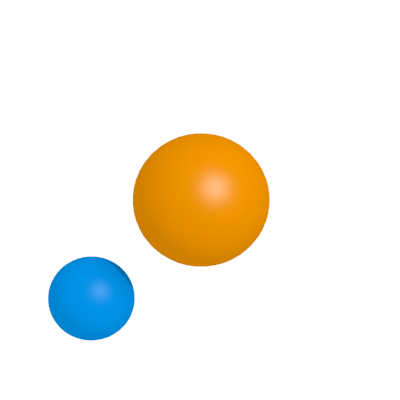
\includegraphics[width=\textwidth]{images/passivation/tetrahedra01.png}
        \caption{}
%         \caption{Illustration of how to divide a convex hexahedron into five tetraheda.}
%         \label{fig:hex_to_tetra}
    \end{subfigure}
%     \hspace{5mm}
    \begin{subfigure}[b]{0.24\textwidth}
        
\includegraphics[width=\textwidth]{images/passivation/tetrahedra02.png}
        \caption{}
%         \caption{A random fracture made from two periodic heightmaps.}
%         \label{fig:fracture_model}
    \end{subfigure}
%     \hspace{5mm}
    \begin{subfigure}[b]{0.24\textwidth}
        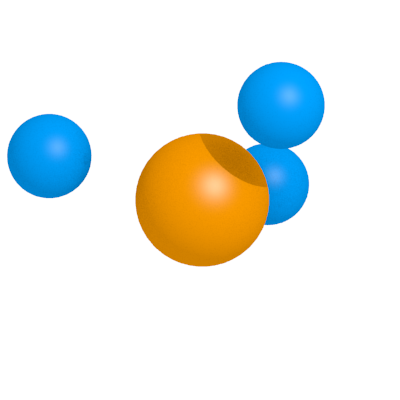
\includegraphics[width=\textwidth]{images/passivation/tetrahedra03.png}
        \caption{}
%         \caption{A random fracture made from two periodic heightmaps.}
%         \label{fig:fracture_model}
    \end{subfigure}
%     \hspace{5mm}
    \begin{subfigure}[b]{0.24\textwidth}
        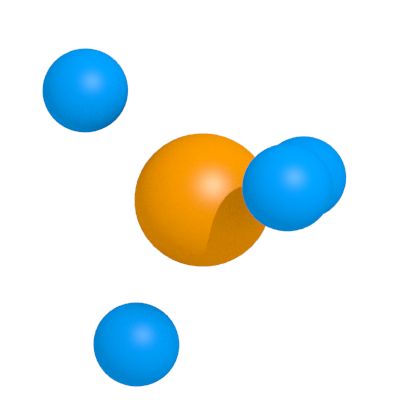
\includegraphics[width=\textwidth]{images/passivation/tetrahedra04.png}
        \caption{}
%         \caption{A random fracture made from two periodic heightmaps.}
%         \label{fig:fracture_model}\caption{}
    \end{subfigure}
    \caption{\hl{Caption}}
    \label{fig:passivation}
\end{figure}

\begin{itemize}
    \item Tetrahedra
    \item Neighbor lists -- see base\_code/passivate\_using\_tetrahedra/passivator.cpp near line 700
    \begin{itemize}
        \item Create list of atoms in each voxel
        \item Create neighbor lists for each atom by looping through neighbor voxels for each atoms
    \end{itemize}
    \item Count number of neighbors of different types -- find number of missing neighbors, Si - 4 Oxygen, Oxygen 2 Si
    \item Insert OH on Si with missing O neighbors, insert H on Oxygen with missing Si neighbors
    \begin{itemize}
        \item Insert O/H at good angles
    \end{itemize}
    \item Improvement: find the atoms near surface using voxels, only passivate those atoms
\end{itemize}

\section{Injecting water}
To fill the pore we have made \hl{(after passivating the system)} we use the technique of \emph{voxelation} (see \cref{sec:voxelation}), and put one water molecule in each unoccupied voxel. The water density is then controlled by the size of the voxels.

If we want to inject water with density $\rho$ [kg/m$^3$], we can find the voxel size we need using the molar mass of water, $M_\text{H$_2$O} = M = 0.0180158 \text{ kg/mol}$. We find the ``volume'' of a water atom in \Ang, the unit used in the \hl{MD integrator/program and output files}, as follows
\begin{align*}
    V 
    &= \frac{ M\text{ [kg/mol]} }{ \rho\text{ [kg/m$^3$]} } \\
    &= \frac{
            M\text{ [kg/mol]} \times \dfrac{1}{N_A \text{ [mol$^{-1}$]}}
        }{
            \rho\text{ [kg/m$^3$]} \times \left(10^{-10} \text{ [\AA/m]}\right)^3
        } \\
    &= \frac{M}{\rho} \times \frac{10^{-30}}{N_A} \text{ [\AA$^3$]},
%     \times \frac{N_A \text{ [mol$^{-1}$]}}{10^{-10} \text{ [\AA/m]}} 10 \text{ [m$^3$]} \\
\end{align*}
from which we find the size we need our voxels to be as
\begin{align*}
    L = \left(\frac{M}{\rho} \times \frac{10^{30}}{N_A}\right)^{1/3}\text{ [\AA]}.
\end{align*}

We then divide the system into voxels of length $L$. And put one water molecule with random orientation in the center of each empty voxel. The naive way of finding the empty voxels is to just find which voxel each existing silicon and oxygen atom is in, and mark those as occupied. But the amorph \hl{structure} of solid silica means that we have a lot of very small pores inside the matrix, which ends up as empty voxels. \todo{something about definition of a pore?}

What we do is to assign a radius to each atom type \todo{which is hard, Si-O, ???}, and mark all voxels with it's center within this radius as occupied.

\begin{itemize}
    \item Voxelize system -- size depends on wanted density
    \item Mark all voxels within distance from other atoms as occupied
    \item Fill other voxels with H2O with random O-H orientation, but correct angle
    \item Improvement: Use one voxel size in the beginning (to avoid one-voxel pores), and then use a smaller voxel size when injecting water
\end{itemize}

\section{Thermostats}

    \chapter{Other measurements???}
% \section{Voxelation, calculating distances, finding neighbors, neighbor lists, periodicity tricks\label{sec:voxelation}}

\section{Measuring as function of distance from matrix}
\todoa{Finish measuring as function of distance from matrix}
% Mean distance from matrix in range --> if we limit the standard deviation as well, we're effectively limiting temperature, or diffusion??
% When measuring things like density, diffusion, and the tetrahedral order parameter in a nanoporous system, we often want to study the behaviour of 

When doing experiments with nanoporous and nanoscale systems we often want to do measures as function of the distance to the surface of the pore, in our case meaning the distance to the interface between water and silica. The first problem with this is to find out how to measure the distance from a point, for example a water molecule, to the surface. Most of our measures are done on water molecules in fractures and pores, so we first define the position of the water molecule as equal to the position of the oxygen atom in the water molecule\footnote{\hl{Something about using positions of hydrogen atoms as well as oxygen position to define water position?}}. We then use the distance from these water-oxygen atoms to the nearest silica atom to define a distance from the water molecule to the surface of the \hl{pore/fracture}. Finding the nearest silica atom isn't trivial, so a procedure for doing this is shown in \cref{sec:find_distance_to_surface}.

When measuring \hl{things} that only depend on data from one timestep we don't have to worry about that the atoms move, so we just sort the atoms by distance to the surface using the procedure in \cref{sec:find_distance_to_surface} and do our measurements, individually on each timestep. But if we want to study for example diffusion, or the tetrahedral order parameter, which depend on data from several timesteps, we have to find a good way to define which atoms are in a certain range of the surface. We tried different methods, but decided to use the average distance to the surface for this\todobo{why, examples of tested methods}.

\section{Voxelation\label{sec:voxelation}}
The method of voxelation is a method where we divide our simulation system into adjacent boxes or \emph{voxels} (3-dimensional pixels). The system is divided into $n_x\times n_y\times n_z$ voxels of size $l_x\times l_y\times l_z$. Depending the what we want to calculate we can calculate the voxel size from the number of voxels, or vice versa, using the following relation
\begin{align*}
    n_i = \frac{L_i}{l_i},
\end{align*}
where $L_i$ is the system size, assuming that the voxel size $l_i$ is set so that $L_i$ is evenly divisible by $l_i$, that the remainder of $L_i/l_i$ is zero. If we have a maximum or minimum voxel size $l_i^\text{max}$ or $l_i^\text{min}$ we can use the following relations to calculate the number of voxels
\begin{align*}
    &n_i=\left\lfloor\frac{L_i}{l_i^\text{max}}\right\rfloor &\text{or}& &n_i=\left\lceil\frac{L_i}{l_i^\text{min}}\right\rceil,
\end{align*}
where $\lfloor x \rfloor$ is the \Verb!floor!-function and $\lceil x \rceil$ is the \Verb!ceil!-function.

The voxels are indexed $(i,j,k)$ where $i,j,k \in [0,n_i-1]$, and a voxel is defined as the points $(x,y,z)$ where
\begin{align}
    \left\lfloor\frac{x}{l_x}\right\rfloor = i,\label{eq:find_voxel_index}
\end{align}
and similarly for the other dimensions.

\subsection{Neighbor lists\label{sec:neighbor_lists}}
When doing calculations and measurements on a molecular system, we often need information about the neighboring atoms of each atom, and we want to make a so-called \emph{neighbor list}, which are lists of which atoms are within a distance $dr$ of each atom. Finding out which atoms are within a certain distance of each atom can take a long time; the trivial way of checking each atom against all other atoms scales as $\mathcal{O}(N^2)$, $N$ being the number of atoms. 
%
%There are many clever algorithms for finding nearest neighbors, often called a ``nearest neighbor search'' (see \url{http://www.slac.stanford.edu/cgi-wrap/getdoc/slac-r-186.pdf} and references in that paper, especially ``11. Levinthal 1966''). 

Since we want to find all neighbors within a distance $dr$ of a point, for all or most of the atoms, we can use the voxelation method to do it efficiently. To do this we first voxelate the system using a minimum voxel size equal to $r$. We then find which voxel each atom belongs to, and store this. We can then find the atoms within a distance $dr$ from a point $(x,y,z)$ by first finding the voxel this point lies in using (from \cref{eq:find_voxel_index})
\begin{align*}
    &i = \Bigg\lfloor \frac{x}{l_x} \Bigg\rfloor,& &j = \Bigg\lfloor \frac{y}{l_y} \Bigg\rfloor,& &j = \Bigg\lfloor \frac{z}{l_z} \Bigg\rfloor,&
\end{align*}
where $l_x\times l_y \times l_z$ is the actual voxel size (we need an even number of voxels, so the actual voxel size is governed by the system size). We then check the distance between the point and the atoms in the voxel the point belongs in, and the atoms in the 26 neighboring voxels of this voxel. 
\todoc{make voxel size vs. $dr$ illustration}%

Checking the 26 neighboring voxels ensure that we included all atoms within the distance $dr$. We can see this by looking at the worst case example, where we have a point right at the edge of the voxel it belongs to, at $(i+(1-\epsilon_0))$, and an atom in voxel $(i+2)$ being as close to the point as possible, at $(i+2 + \epsilon)$. The distance between those two points would then be
\begin{align*}
    ((i+2)l + \epsilon_1) - (il + (l-\epsilon_0)) 
    &= ((i + 2) - (i + 1) - \epsilon_0)l + \epsilon_1 + \epsilon_0 \\
    &= l + \epsilon + \epsilon_0,
\end{align*}
which is larger than $l$, since $\epsilon_0, \epsilon_1$ have to be larger than 0.

When voxelating the system using the distance $r$ we should take care not to use a too small distance, i.e. make the voxels too small and create a lot of voxels. Since the total number of voxels goes as $n^3$ the memory needed to store the matrix increases rapidly with decreasing voxel size. To avoid this we usually implement a hard limit to the number of voxels, and found that a limit of $n < 256$ or even $n < 128$ seemed to work good in most cases. On the other hand, if we make the voxels too large we soon find that the program isn't especially efficient. This is because most voxels will have a lot of atoms in then, and we have to look through a lot of atoms when checking the 26+1 voxels for each atom.

An implementation of the voxelation method for creating neighbor lists can be seen in \cref{list:create_neighbor_lists}. Note that when calculating distances between points we usually calculate and compare squared distances like $r^2 = (x_1-x_2)(x_1-x_2) + \dots$, since calculating roots are a time-consuming operation on a computer (at least compared to multiplication and addition).
%
% We didn't find any algorithms for solving this specific problem, and the usual algorithms can't benefit from the fact that we need to find the nearest neighbors of \emph{all} points.
%
\begin{listing}[!htb]%
\begin{cppcode*}{gobble=4}
    int nVoxels = floor(systemSize/radius);
    double voxelSize = systemSize*nVoxels;
    
    sortAtomsIntoVoxels(atoms, voxelSize, voxels);
    
    vector<vector<Atom*> > neighborAtoms(atoms.size());
    
    // Loop over all atoms
    for (Atom *atom : atoms)
    {
        // Index of the voxel this atom belongs to
        ivec3 index = floor(atom.position() / voxelSize)
        
        // Loop over all 27 neighbor voxels (including self)
        for (int di = -1; di <= 1; di++)
        for (int dj = -1; dj <= 1; dj++)
        for (int dk = -1; dk <= 1; dk++)
        {{{
            // Index of neighbor voxel using periodic boundary conditions
            // nx, ny, nz is the number of voxels in each direction
            int i = (index[0] + di + nx) % nx;
            int j = (index[1] + dj + ny) % ny;
            int k = (index[2] + dk + nz) % nz;
            
            neighborAtoms[atom.index()].push_back(
                findAtomsWithinRadius(atom, voxels[i][j][k], radiusSquared)
            );
        }}}
    }
\end{cppcode*}
\caption{%
    An example of how to find the neighbor atoms within a given distance (\texttt{radius}) of all atoms. This example assumes a cubic system of size \texttt{systemSize}. See \cref{list:sortAtomsIntoVoxels,list:findAtomsWithinRadius} for example implentations of \texttt{sortAtomsIntoVoxels} and \texttt{findAtomsWithinRadius}. %
    \label{list:create_neighbor_lists}%
}%
\end{listing}%
%
\begin{listing}[!htb]%
\begin{cppcode*}{gobble=4}
    void sortAtomsIntoVoxels(
        const vector<Atom*> &atoms, 
        double voxelSize, 
        vector<vector<vector<Atom*> > > &voxels)
    {
        for (Atom *atom : atoms)
        {
            // Index of the voxel this atom belongs to
            int i = floor(atom.position().x() / voxelSize);
            int j = floor(atom.position().y() / voxelSize);
            int k = floor(atom.position().z() / voxelSize);
            voxels[i][j][k].push_back(atom);
        }
    }
\end{cppcode*}
\caption{%
    Example implementation of the procedure detailed in \cref{somesection}, to sort atoms into voxels of size \texttt{voxelSize}. We use the \texttt{floor} function to get the index of the voxel each atom belongs in, using zero-based numbering. % \texttt{sortAtomsIntoVoxels}. %
    \label{list:sortAtomsIntoVoxels}%
}%
\end{listing}%
\begin{listing}[!htb]%
\begin{cppcode*}{gobble=4}
    vector<Atom*> findAtomsWithinRadius(
        Atom *atom1, const vector<Atom*> &voxel, double radiusSquared)
    {
        vector<Atom*> neighborAtoms;
        
        // Loop over atoms in neighbor voxel
        for (Atom *atom2 : voxel)
        {
            if (atom2 != atom1)
            {
                double drSquared = 
                    calculateDistanceSquaredBetweenAtoms(atom1, atom2);
                if (drSquared < radiusSquared)
                {
                    neighborAtoms.push_back(atom2);
                }
            }
        }
        return neighborAtoms;
    }
\end{cppcode*}
\caption{%
    \texttt{findAtomsWithinRadius}. See \cref{list:calculateDistanceSquaredBetweenAtoms} for an example implementation of \texttt{calculateDistanceSquaredBetweenAtoms}.%
    \label{list:findAtomsWithinRadius}%
}%
\end{listing}%
%
\begin{listing}[!htb]%
\begin{cppcode*}{gobble=4}
    double calculateDistanceSquaredBetweenAtoms(Atom *atom1, Atom *atom2)
    {
        vec3 dr = atom2->position() - atom1->position();
        
        // Minimum image convention
        for (int dim = 0; dim < 3; dim++)
        {
            if      (dr[dim] >  L[dim]/2.0) dr[dim] -= L[dim];
            else if (dr[dim] < -L[dim]/2.0) dr[dim] += L[dim];
        }
        
        // Calculate $dr^2$ instead of $\sqrt{dr^2}$, since sqrt() is a very 
        // slow operation, and in this case is unnecessary
        return dr.lengthSquared();
    }
\end{cppcode*}
\caption{%
    \texttt{calculateDistanceSquaredBetweenAtoms}%
    \label{list:calculateDistanceSquaredBetweenAtoms}%
}%
\end{listing}%

\subsection{Finding distance to surface\label{sec:find_distance_to_surface}}
When doing measurements on water molecules we often want to know the distance from the water molecule to the surface of the pore the water molecule is in. To find this we first define the position of the water molecule as the position of the oxygen atom in the molecule. We then use the distance between this oxygen atom to the nearest silicon atom as the distance to the surface.

To use the voxelation method we need to have a maximum distance to look for silicon atoms in. This atom should be set as small as possible, to efficiently use the voxelation method\footnote{We usually implement a hard upper bound on the number of voxels, or a lower bound on the voxel size, to keep the memory consumption of our program in check}. We divide the system into voxels using the technique from \cref{sec:voxelation}, and sort all silicon atoms into the voxels. For each water-oxygen atom we then find the distance to the nearest silicon atom by calculating the distance between the oxygen atom and the silicon atoms in the voxel the oxygen atom belongs in, and the silicon atoms in all 26 neighbor voxels. See \cref{sec:neighbor_lists} for more details.

% To use the voxelation technique for finding the nearest atom we need to set a maximum distance we want to look for silicon atoms in. This distance should be set large enough that we get the results we want, but at the same time it should be as small as possible, to increase the efficiency of the voxelation method. If we set the voxel size very large most voxels will have a lot of atoms in them, and we have to look through a lot of atoms to find the nearest one.

% should not be set too large, as this will decrease performance, since then most voxels will have a lot of atoms in them, and we have to loop over a lot of atoms to find the nearest one. Sometimes we need to look within a large distance though, and have to live with this cost.

% \section{Voxelation\label{sec:voxelation}}
% Our solution to the problem is inspired by the ``cell list'' method used in MD integrators\hl{(see Frenkel Appendix F)}, and uses a method we call ``voxelation''/\emph{voxelation}. This method divides the system into $n_x \times n_y \times n_y$ boxes, or 3-dimensional pixels, called \emph{voxels}, with $n_i$ voxels in each direction. We then sort all atoms into their respective voxels (usually implemented using a list of indexes or pointers to objects in \cpp). To find the index ($i,j,k$) of the voxel each atom belongs to, we use the \Verb!floor! function \hl{($\lfloor \rfloor$)}
% \begin{align*}
%     &i = \Bigg\lfloor \frac{x}{l_x} \Bigg\rfloor,& &j = \Bigg\lfloor \frac{y}{l_y} \Bigg\rfloor,& &j = \Bigg\lfloor \frac{z}{l_z} \Bigg\rfloor,&
% \end{align*}
% where $l_i$ is the size of the voxels in each direction, and ($x,y,z$) is the position of the atom. Here we use zero-based numbering. See \cref{list:sortAtomsIntoVoxels} for an example of an algorithm that sorts the atoms into their respective voxels.
% % %
% % \begin{listing}[!htb]%
% % \begin{cppcode*}{gobble=4}
% %     void sortAtomsIntoVoxels(
% %         const vector<Atom*> &atoms, 
% %         double voxelSize, 
% %         vector<vector<vector<Atom*> > > &voxels)
% %     {
% %         for (Atom *atom : atoms)
% %         {
% %             // Index of the voxel this atom belongs to
% %             int i = floor(atom.position().x() / voxelSize);
% %             int j = floor(atom.position().y() / voxelSize);
% %             int k = floor(atom.position().z() / voxelSize);
% %             voxels[i][j][k].push_back(atom);
% %         }
% %     }
% % \end{cppcode*}
% % \caption{%
% %     Example implementation of the procedure detailed in \cref{somesection}, to sort atoms into voxels of size \texttt{voxelSize}. We use the \texttt{floor} function to get the index of the voxel each atom belongs in, using zero-based numbering. % \texttt{sortAtomsIntoVoxels}. %
% %     \label{list:sortAtomsIntoVoxels}%
% % }%
% % \end{listing}%
% 
% When creating the voxels we should look out for very small voxel sizes compared to the system size. Since the number of voxels scale as $n^3$, $n$ being the number of voxels in each direction (in a cubic system), we soon run in to memory problems on a computer if we try to use a lot of voxels. To avoid this we can implement a minimum voxel size, or a maximum number of voxels. We found that limiting the number of voxels to $n \leq 256$ or even $n \leq 128$ seemed to work well in most cases, but this depends heavily on the simulated system and the available memory on the computer.
% 
% \subsection{Finding nearest neighbors}
% If we want to find all neighbors within a radius $dr$ we can divide the system into voxels of size $l \geq dr$ and sort the atoms into their respective voxels. See \cref{list:sortAtomsIntoVoxels} for an example of how to do this. To get an integer number of voxels, while ensuring that we use large enough voxels, we use the \Verb!floor! function \hl{($\lfloor \rfloor$)} to calculate the number of voxels $n_i$ we should use in each direction
% \begin{align*}
%     n_i = \left\lfloor \frac{L_i}{dr} \right\rfloor,
% \end{align*}
% where $L_i$ is the system size in each direction. We then calculate the size of the voxels in each direction $l_i$ from the number of voxels using
% \begin{align*}
%     l_i = L_i*n_i.
% \end{align*}
% 
% For an atom at position $\rvec$ we can now find the \hl{neighboring} atoms within the radius $dr$ by finding which voxel the atoms belongs to, and checking the distance between the atom and all atoms in that voxel, and between and all atoms in the 26 neighboring boxes\todo{replace all ``box'' with ``voxel'' ?}. See \cref{list:check_neighbor_voxels} for an example of how to find neighbor atoms using this method.


% \begin{listing}[!htb]%
% \begin{cppcode*}{gobble=4}
%     int nVoxels = floor(systemSize/radius);
%     double voxelSize = systemSize*nVoxels;
%     
%     sortAtomsIntoVoxels(atoms, voxelSize, voxels);
%     
%     vector<vector<Atom*> > neighborAtoms(atoms.size());
%     
%     // Loop over all atoms
%     for (Atom *atom : atoms)
%     {
%         // Index of the voxel this atom belongs to
%         ivec3 index = floor(atom.position() / voxelSize)
%         
%         // Loop over all 27 neighbor voxels (including self)
%         for (int di = -1; di <= 1; di++)
%         for (int dj = -1; dj <= 1; dj++)
%         for (int dk = -1; dk <= 1; dk++)
%         {{{
%             // Index of neighbor voxel using periodic boundary conditions
%             // nx, ny, nz is the number of voxels in each direction
%             int i = (index[0] + di + nx) % nx;
%             int j = (index[1] + dj + ny) % ny;
%             int k = (index[2] + dk + nz) % nz;
%             
%             neighborAtoms[atom.index()].push_back(
%                 findAtomsWithinRadius(atom, voxels[i][j][k], radiusSquared)
%             );
%         }}}
%     }
% \end{cppcode*}
% \caption{%
%     An example of how to find the neighbor atoms within a given distance (\texttt{radius}) of all atoms. This example assumes a cubic system of size \texttt{systemSize}. See \cref{list:sortAtomsIntoVoxels,list:findAtomsWithinRadius} for example implentations of \texttt{sortAtomsIntoVoxels} and \texttt{findAtomsWithinRadius}. %
%     \label{list:create_neighbor_lists}%
% }%
% \end{listing}%

% \begin{listing}[!htb]%
% \begin{cppcode*}{gobble=4}
%     vector<Atom*> findAtomsWithinRadius(
%         Atom *atom1, const vector<Atom*> &voxel, double radiusSquared)
%     {
%         vector<Atom*> neighborAtoms;
%         
%         // Loop over atoms in neighbor voxel
%         for (Atom *atom2 : voxel)
%         {
%             if (atom2 != atom1)
%             {
%                 double drSquared = 
%                     calculateDistanceSquaredBetweenAtoms(atom1, atom2);
%                 if (drSquared < radiusSquared)
%                 {
%                     neighborAtoms.push_back(atom2);
%                 }
%             }
%         }
%         return neighborAtoms;
%     }
% \end{cppcode*}
% \caption{Test%
%     \texttt{findAtomsWithinRadius}. See \cref{list:calculateDistanceSquaredBetweenAtoms} for an example implementation of \texttt{calculateDistanceSquaredBetweenAtoms}.%
%     \label{list:findAtomsWithinRadius}%
% }%
% \end{listing}%
% 
% \begin{listing}[!htb]%
% \begin{cppcode*}{gobble=4}
%     double calculateDistanceSquaredBetweenAtoms(Atom *atom1, Atom *atom2)
%     {
%         vec3 dr = atom2->position() - atom1->position();
%         
%         // Minimum image convention
%         for (int dim = 0; dim < 3; dim++)
%         {
%             if      (dr[dim] >  L[dim]/2.0) dr[dim] -= L[dim];
%             else if (dr[dim] < -L[dim]/2.0) dr[dim] += L[dim];
%         }
%         
%         // Calculate $dr^2$ instead of $\sqrt{dr^2}$, since sqrt() is a very 
%         // slow operation, and in this case is unnecessary
%         return dr.lengthSquared();
%     }
% \end{cppcode*}
% \caption{%
%     \texttt{calculateDistanceSquaredBetweenAtoms}%
%     \label{list:calculateDistanceSquaredBetweenAtoms}%
% }%
% \end{listing}%

% \section{Mean square displacement} % - in ensemble chapter?
% \section{Density} % - in ensemble chapter?
% \section{Diffusion} % - in ensemble chapter?

\FloatBarrier
\section{Density}
To measure the density in a uniform system consisting of just one atom type, we can use
\[
    \rho = \frac{Nm}{V},
\]
where $N$ is the number of atoms, $m$ the mass of an atom, and $V$ the volume of the whole system. But if we have a more complicated system, like in our case where we have three different atom types, liquid water in some parts of the system, and solid silica in other parts, we can't use that simple relation. What we do instead is to assiociate a volume $V_i^j$ with each atom of type $j$, and calculate the density of atom type $j$ using
\[
    \rho_j = \dfrac{m_jM}{\sum_{i=0}^M V_i^j},
\]
where $m_j$ is the mass an atom of type $j$, and $M$ is the number of atoms of type $j$. \hl{We identify as the $\rho_j/m_j$ number density.} We can find the mass of an atom type from standard tables of molar masses, but we still need to find the volumes $V_i^j$ associated with each atom. To do this we use something called \hl{Voronoi cells/Voronoi tesselation}\todo{citation? Dirchlet 1850 and Voronoi 1908, so very old...}. Voronoi tesselation is done by dividing the system into non-overlapping convex polyhedra (or convex polygons in 2 dimensions), with one atom in each polyhedra. The volume inside the polyhedron surrounding each atom consists of all points in space closer to that atom than any other atom. See \cref{fig:2d_voronoi_diagram} for an illustration of a 2-dimensional Voronoi, and \cref{fig:3d_voronoi_diagram} for a rendering of a 3D Voronoi diagram.
%
\begin{figure}%
% \centering%
    \begin{minipage}[t]{0.485\textwidth}%
        \captionsetup{width=\textwidth}%
        \centering%
%         \includesvg[width=0.8\textwidth, svgpath=./images/voronoi/]{2d_diagram03}%
        \includesvg[height=0.7\textwidth, svgpath=./images/voronoi/]{2d_diagram04}%
        \caption{%
            Illustration of Voronoi cells in 2 dimensions. Freely after Wikipedia Commons\cite{wikiVoronoiImage}.%
            \label{fig:2d_voronoi_diagram}%
        }%
    \end{minipage}%
    \hfill%
    \begin{minipage}[t]{0.485\textwidth}% % change "b" to "t" to anchor top instead of bottom
    \captionsetup{width=\textwidth}% % minipage defines a \textwidth for it's own, so we have to repeat this command inside the minipage
        \centering%
%         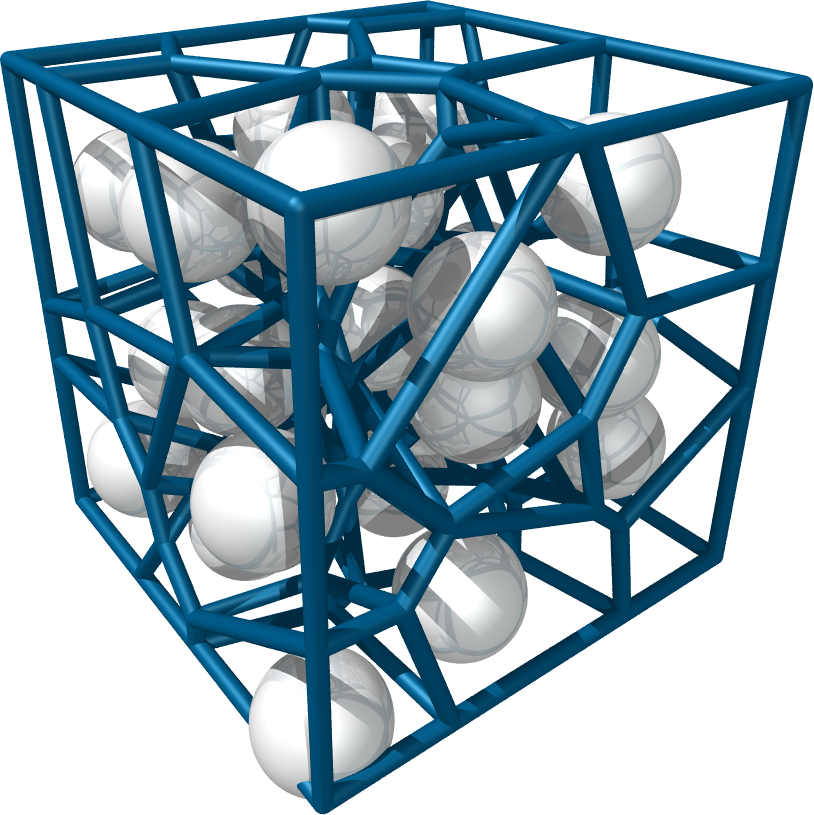
\includegraphics[width=0.8\textwidth]{images/voronoi/3d_diagram04_crop.png}%
        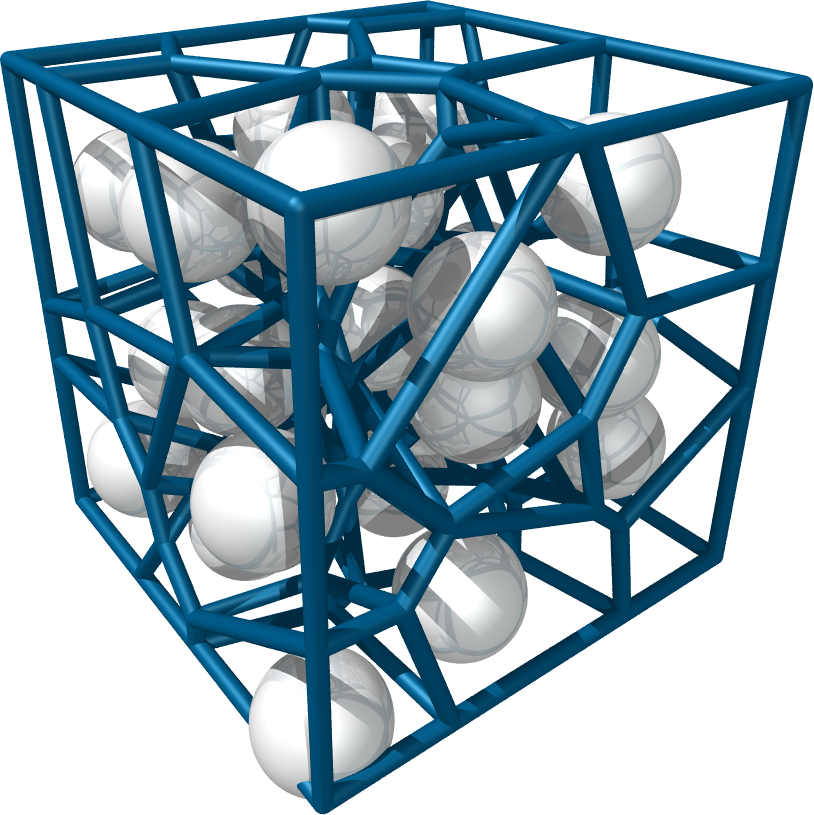
\includegraphics[height=0.7\textwidth]{images/voronoi/3d_diagram04_crop.png}%
        \caption{%
            Rendering of Voronoi cells in 3 dimensions, in a system of 27 particles. Voronoi cells created using the \cpp-library \texttt{Voro++}\cite{rycroft2009voro,webvoro++}, and rendered using the program \texttt{povray}\cite{webpovray}. %
            \label{fig:3d_voronoi_diagram}%
        }%
    \end{minipage}%
\end{figure}%

\todob{Something about removing hydrogen atoms, and just use oxygen position as hydrogen position, and water atom ``volume''? This simplifies life for us, since we don't have to find which water molecule each hydrogen atom belongs to, but we could get inconsistent water density. But since we use the same method for all measurements, we can compare relative densities.}

\todob{Something about removing extreme points/tail in distribution? Caused by vacuum.}

\section{Diffusion}
\todob{derivation of diffusion? See \cite[Section~4.4.1]{frenkel2001understanding}}
When we talk about diffusion in \hl{the context of} this thesis we mean the process of \emph{self-diffusion}, which is different from \hl{``normal''} diffusion which is the net movement of a substance in the presence of a gradient, which can be for example a concentration gradient, a temperature gradient, or a pressure gradient. With \emph{self-diffusion} we mean the \hl{random?} movement in a substance that has no gradients.

Diffusion can be characterized by a constant $D$, which is related to the displacement of each atom relative to a initial position. We can measure this constant by measuring the mean square displacement $r_i^2(t)$ of each atom as a function of time, and average over all atoms. The mean square displacement is measured as
\begin{align*}
    \Braket{r^2(t)} = \frac{1}{N} \sum_{i=1}^N \left( \rvec_i(t) - \rvec_i(t=0) \right)^2,
\end{align*}
where $\rvec_i(t=0)$ is the initial position of atom $i$. From theoretical considerations of the diffusion process we can relate the diffusion constant to the mean square displacement through\cite[Section~4.4.1]{frenkel2001understanding}
\begin{align}
    \lim_{t\rightarrow \infty}\dpd{}{t}\Braket{r^2(t)} = 2dD\label{eq:diffusion_derivative}
\end{align}
where $d$ is the \hl{spatial} \hl{dimensionality/dimension?}. This means that we can find the diffusion constant in a molecular dynamics simulation by measuring the mean square displacement for many timesteps, and find the slope of this data as the diffusion constant in the limit $t\rightarrow \infty$. \hl{We are limited in that we can't actually simulate infinite number of timesteps, but have to find a reasonable number of timesteps to measure over.} An example of how to sample the mean square displacement $\Braket{r^2(t)}$ in a simulation can be seen in \cref{list:diffusionSample}.
%
% This means that we can find the diffusion constant in a molecular dynamics simulation by measuring the mean square displacement for many timesteps, and plotting $\Braket{r^2(t)}/(2dt)$ as a function of time. The diffusion constant will then be the value this expression approaches when simulating for enough timesteps.
%
%An example of how to measure the mean square displacement in a molecular dynamics \hl{simulation/program} as outlined in \cref{chap:simple_md_program} can be seen in \cref{list:diffusionSample}.
% Fick's law relates flux $\bvec j$ of diffusing species to the concentration gradient $\bvec \nabla c$ of the species
% \begin{align*}
%     \bvec j = -D\bvec \nabla c,
% \end{align*}
% where $D$ is the proportionality constant called the diffusion \hl{coefficient/constant}.
% 
% Conservation of \hl{species/atoms?}
% \begin{align*}
%     \dpd{c(r,t)}{t} + \div \cdot \vec j(r,t) = 0,
% \end{align*}
% which gives
% \begin{align}
%     \dpd{c(r,t)}{t} - D\nabla^2 c(r,t) = 0.
%     \label{eq:diffusion_diff}
% \end{align}
% % We can solve this equation with the boundary condition
% % \begin{align*}
% %     c(r,0) = \delta (r),
% % \end{align*}
% % where $\delta(r)$ is the Dirac delta function, which gives
% % \begin{align*}
% %     c(r,t) = \frac{1}{(4\pi Dt)^{d/2}} \exp\left(-\frac{r^2}{4Dt}\right).
% % \end{align*}
% By multiplying \cref{eq:diffusion_diff} by $r^2$ and integrating over all space we get
% \begin{align*}
%     \dpd{}{t}\int \drvec~ r^2 c(r,t) = D\int \drvec~ r^2 \nabla^2 c(r,t).
% \end{align*}
% We recognize the integral on the left-hand side as the the mean square displacement %\hl{time dependence of the second moment of $c(r,t)$???}
% \todo{what???}
% \begin{align*}
%     \int \drvec~ c(r,t) r^2 \equiv \Braket{r^2(t)},
% \end{align*}
% where we have imposed
% \begin{align*}
%     \int \drvec~ c(r,t) = 1.
% \end{align*}
% Applying partial integration to the right-hand side we obtain
% \begin{align*}
%     \dpd{\Braket{r^2(t)}}{t} 
%     &= D\int \drvec~ r^2 \nabla^2 c(r,t) \\
%     &= D\int \drvec~ \div \cdot \left(r^2\nabla c(r,t)\right) - D\int\drvec~ \div r^2 \cdot \nabla c(r,t) \\
%     &= D\int \dif \vec S~ \left(r^2\div c(r,t)\right) - 2D\int\drvec~ \rvec \cdot\div c(r,t) \\
%     &= 0 - 2D\int\drvec~ (\div \cdot \rvec c(r,t)) + 2D\int\drvec~ (\div \cdot \rvec) c(r,t) \\
%     &= 0 + 2dD\int \drvec~ c(r,t) \\
%     &= 2dD
% \end{align*}
% 
% 
% \begin{align*}
%     \dpd{\Braket{r^2(t)}}{t} = 6D
% \end{align*}
% $\Rightarrow$ Plot mean square distance as function of time
% \begin{align*}
%     \Braket{\delta r(t)^2} = \frac{1}{N} \sum_{i=1}^N \delta \rvec_i(t)^2
% \end{align*}
% and find $6D$ as slope of plot \hl{(after a while?)}
%
\begin{listing}[!htb]%
\begin{cppcode*}{gobble=4}
    double diffusionSample(System &system)
    {
        double rSquared = 0.0;
        for (Atom *atom : system.atoms())
        {
            drVec = atom->positiom() - atom->initialPosition() 
                    + atom->getBoundaryCrossings()*system.size();
            rSquared += drVec.lengthSquared();
        }
        rSquared /= system.nAtoms();
        return rSquared;
    }
\end{cppcode*}
\caption{%
    An example of how to calculate the mean square displacement in a molecular dynamics simulation. Example implementation of \texttt{diffusionSample} from \cref{list:sampling}. We store the inital positions of the atoms as \texttt{atom->initialPosition()}, and when using periodic boundary conditions we count the number of times we have to translate the atom one system-size in each direction, so while the position of the atom will always be inside the system, the \hl{\emph{real}} position of the atom can be calculated by adding \texttt{atom->getBoundaryCrossings()*system.size()} to $\rvec$.%
    \label{list:diffusionSample}%
}%
\end{listing}%

% To improve our statistics when measuring the diffusion constant as function of distance to the surface of the pore we can use different time origins to get different samples. %
To measure $D$ we see from \cref{eq:diffusion_derivative} that we have to let $t\rightarrow \infty$, but in practice we see that the gradient of $\Braket{r^2(t)}$ usually stabilizes near its final value after ${\sim} 2\text{ k}$ timesteps. We can use this to get more samples for our measurements, by using different time origos. This means that when we have saved a number of states at \todoao{Finish diffusion time origo stuff}

% \FloatBarrier
\section{Tetrahedral order parameter}
The tetrahedral order parameter\cite{errington2001relationship} is effectively a measure of how tetrahedral a \hl{molecule?} is. The tetrahedral order parameter $Q$ for a molecule $k$ is calculated as follows
\begin{align*}
    Q_k = 1 - \frac{3}{8}\sum_i^3\sum_{j=i+1}^4 \left[ \cos \theta_{ikj} + \frac{1}{3} \right]^2,
\end{align*}
where $\theta_{ikj}$ is the angle between two vectors from the main molecule, $k$, to respectively atom $i$ and atom $j$, and the two sums go over the 6 possible angles $\theta_{ikj}$, between the main molecule and \hl{its} four nearest neighbors. See \cref{fig:top_tetrahedra} for an illustration of the angles and molecules involved in the calculation.
%
\begin{figure}[htpb]%
    \centering%
    \includesvg[width=0.3\textwidth, svgpath=./images/tetrahedral_order_parameter/]{tetrahedra02}%
    \caption{%
        Illustration of the angles and molecules involved in the calculation of the tetrahedral order parameter. The \hl{blue} dots are molecules, in our case usually water molecules. We have the center molecule $k$, and \hl{its} four nearest neighbors. $\theta_{ikj}$ is the angle between molecule $i$, $k$ and $j$, as indicated by the \hl{orange} arc. \hl{FINISH CAPTION}. %
        \label{fig:top_tetrahedra}%
    }%
\end{figure}%

% \FloatBarrier
\section{``Distance to atom''\label{sec:distance_to_atom}}
To help visualize, and to characterize our nanoporous system we developed a program that creates a 3d map of the distance to the nearest atom, in each point in space on a regular grid. The implementation of this program is almost straighforward, but since we have to do a lot of calculations if we want to have a map with decent resolution, we have also parallellized the program. 
\todoa{Write about distance to atom}
\todoc{Distance to atom code example?}

% \FloatBarrier
\section{``Generation matrix''}
Since the program from \cref{sec:distance_to_atom} takes a long time to run to get decent maps with high resolution, we decided to also develop a similar program that creates a 3d map of the space. To ease calculation we this time used a method inspired by the voxelation technique from \cref{sec:voxelation}. This program first divides the system into $n_x\times n_y\times n_z$ voxels, and make a 3d matrix of the same size for storing the label of each voxel. We first give all voxels with one or more atoms in them the label \hl{``0''}. We then label the rest of the voxels using an iterative method, increasing the \hl{numbers/labels} for each iteration. In each iteration we find the voxels that have a neighbor voxel \hl{labelled} with the previous label (\texttt{label-1}), using 4-neighbor connectivity, and give them the current label. When all voxels are labelled, they should have a label corresponding to the \hl{Manhattan distance} to the nearest atom.

Although the Manhattan distance isn't as useful as the regular Euclidean distance we calculate using the \hl{``distance to atom''}-program, the benefit is that making a 3d map of space using the \hl{``generation matrix''} method uses about 3\% of the time that ``distance to atom'' uses for the same system and same resolution. 

\todoa{Something about the usefulness of this measure?}

\orangebox{A system of 347176 atoms (\texttt{rough\_fracture03}), water and SiO2, $256^3$ voxels, $~5$ seconds for ``generation matrix'', 2m27seconds for ``distance to atom'' (on one cpu)}
\todoc{Voxel counter code example?}

% \FloatBarrier
\section{``Voxel counter''}
\todob{Write about voxel counter}
\todod{Voxel counter code example?}
    A histogram of the fraction of voxels that has one or more atom in them vs. the voxel size in x-, y-, and z-direction.
    
% \FloatBarrier
\section{Cage cage correlation}
    \todod{Measure cage cage correlation}

% \FloatBarrier
\section{Surface area of pores}
    Only one large pore in my system, so not useful?


\part{Fractures}
    % \chapter{Fractures}
% \chapter{Introduction}
\vspace*{\fill}
\begin{figure}[hp!]%
\thispagestyle{empty}
    \centering%
    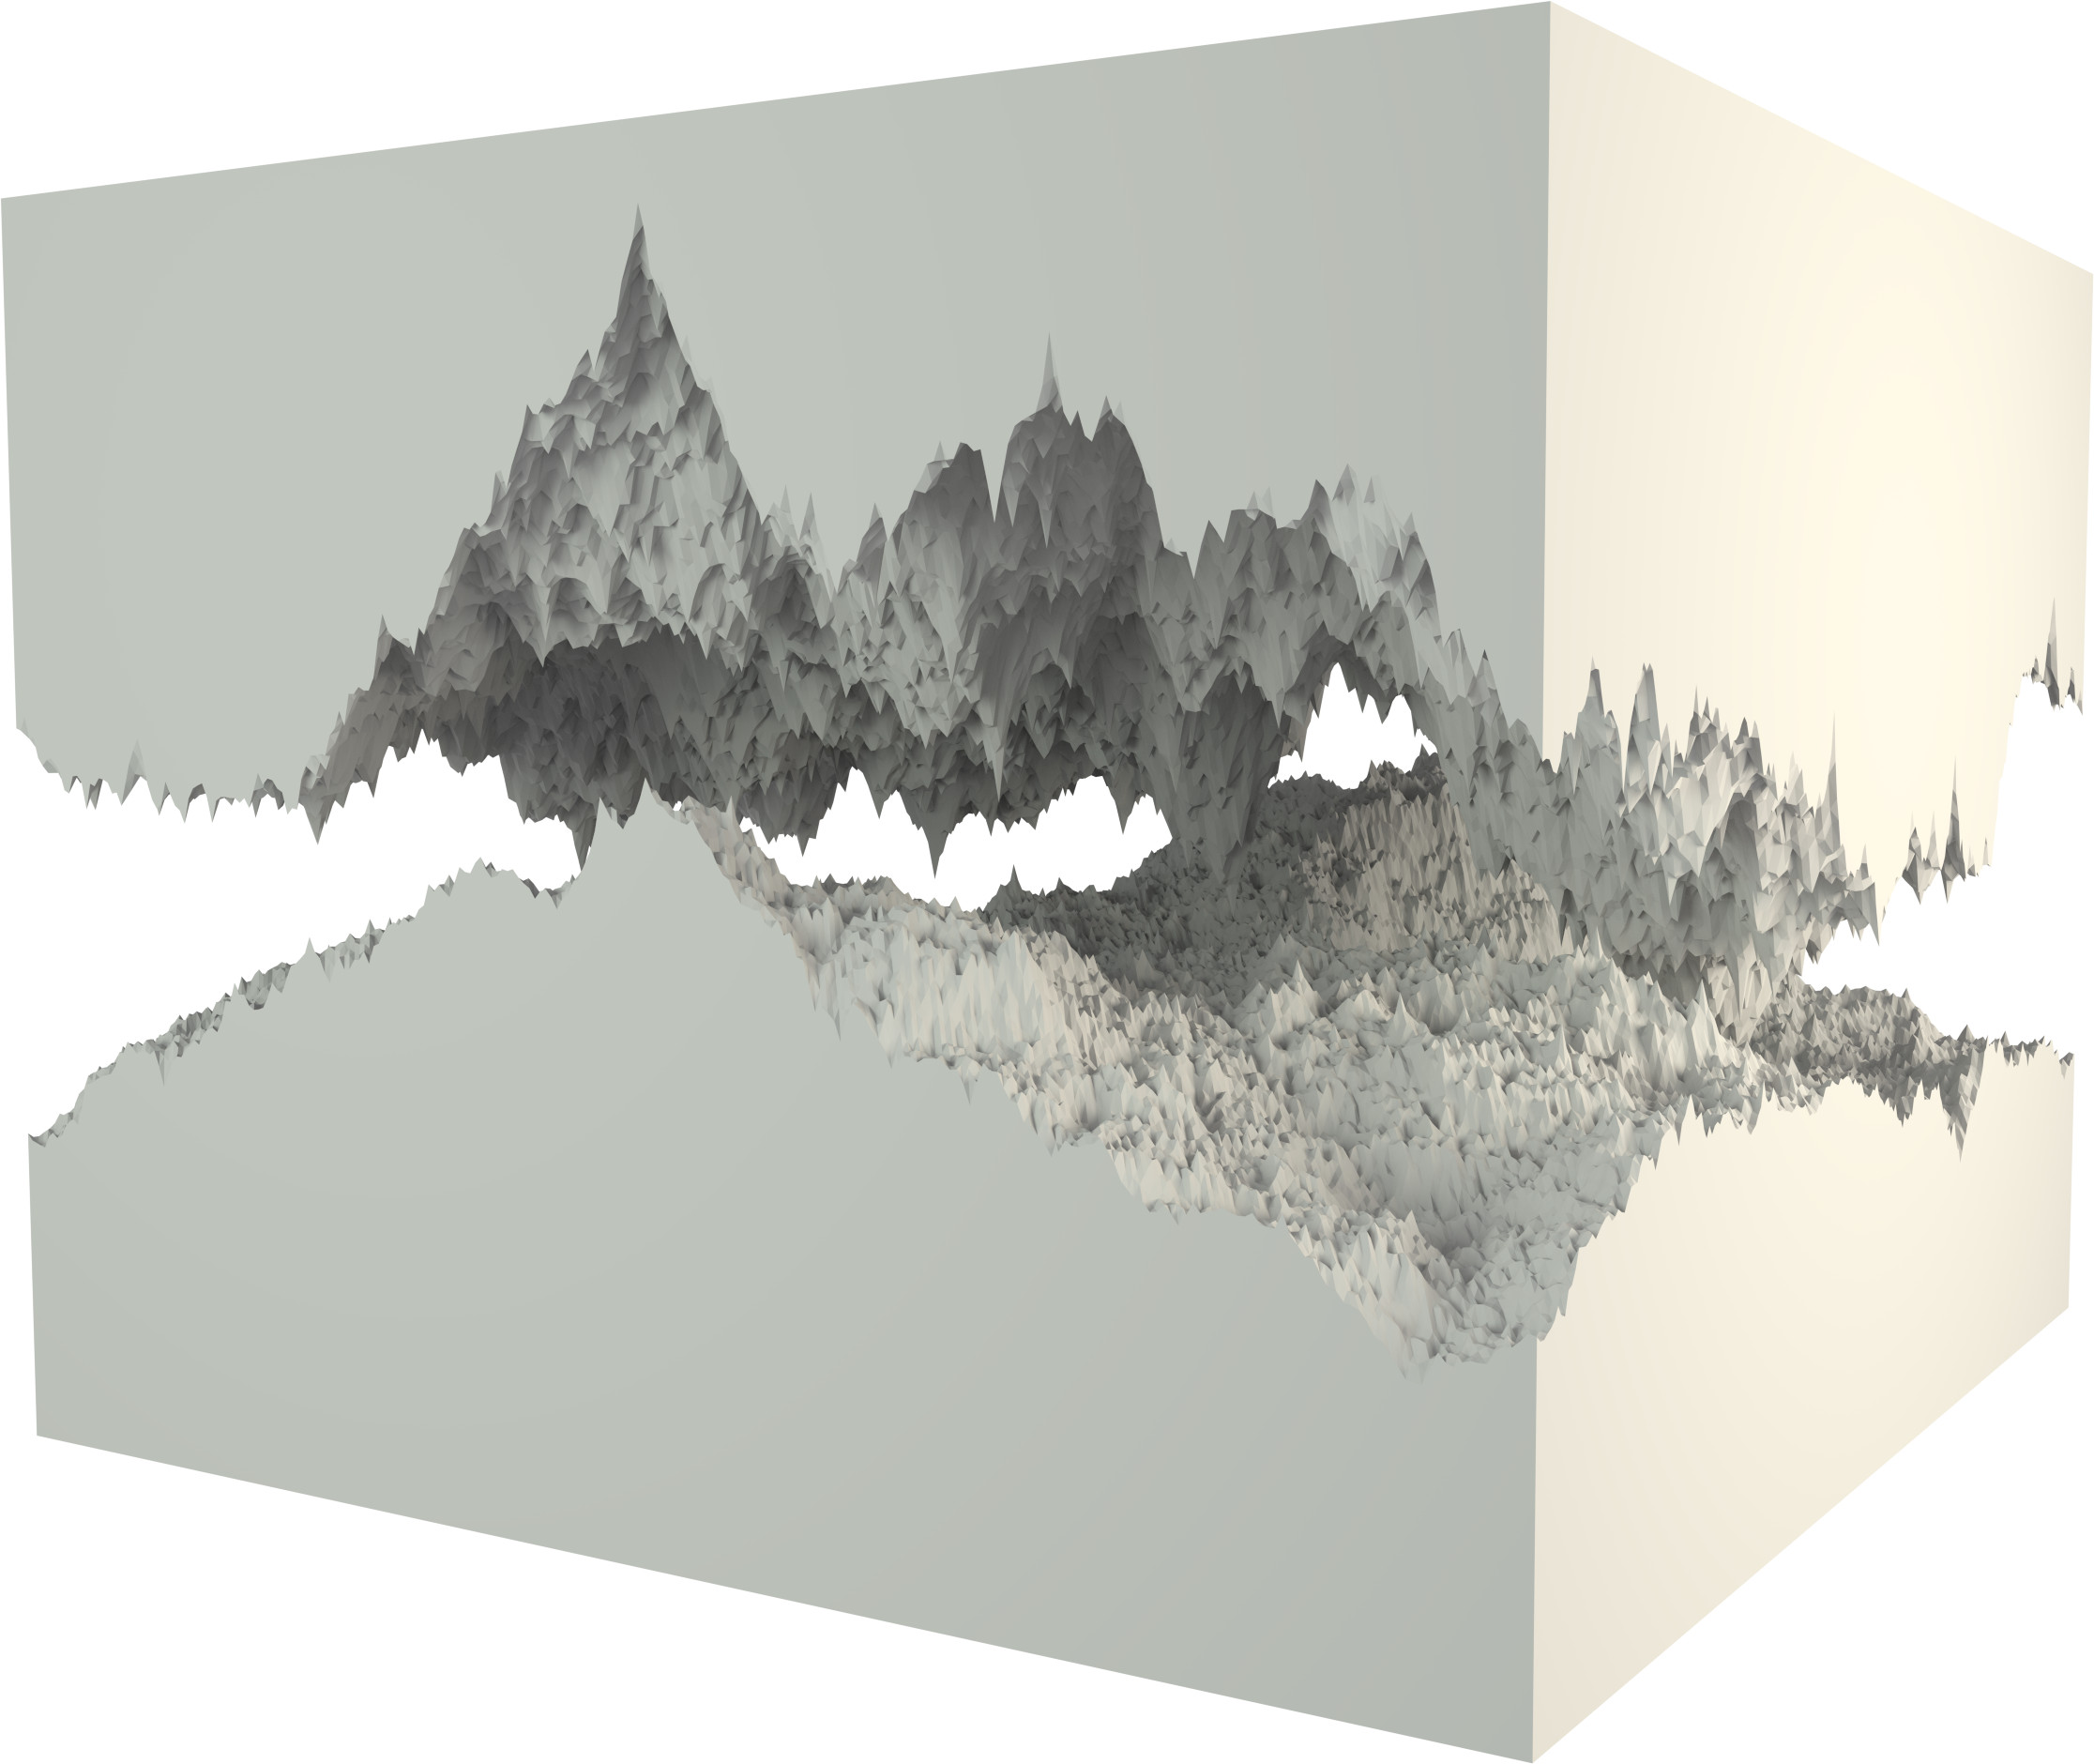
\includegraphics[width=\textwidth]{images/fracture/large_fracture05.jpg}%
    \caption{%
        A randomly generated fracture.%
    }%
\end{figure}%
\vspace{\fill}

\chapter{Introduction}
We want to study the behaviour of water trapped in nanoscale pores and fractures in silica, so need a way to generate and characterize such structures. We choose to model a fracture as two surfaces, with the volume between the surfaces as the void fraction. This makes it easier to make fractures, since we only need to create two surfaces to get a fracture. To generate realistic surfaces we could have used scans of the structures we want to simulate, but the problem with this approach is that the resulting fracture will depend a lot on how we interpret the image, and that we can not easily generate a lot of samples of surfaces. To avoid this we use fractals to describe surfaces, and use this to randomly generate surfaces and fractures that are statistically similar to real fractures. Like a lot of phenomena in nature, fractures and surfaces can be very well described by the theory of fractals\cite{mandelbrot1983fractal}, so we think that this method should give good results.

What makes a \emph{fractal} fractal, or what characterizes a fractal, does not have a rigorous definition, but in general a fractal is something that looks similar to itself at different length scales. A fractal might be \emph{identical} to itself at different length-scales \hl{(self-similar)}, or be \emph{statistically similar} to itself \hl{(statistically self-similar)}. In one dimension this looks like \todoao{Examples of 1D, scale x and y equally for self-similar, different scaling for self-affine}

Fractals and concepts similar to fractals have been discussed as early as the 17th century, but the use of fractals in natural sciences didn't really \hl{take off} before computers became \hl{readily} available and Benoit Mandelbrot gathered and developed a lot of theory on fractals in ``The Fractal Geometry of Nature''\cite{mandelbrot1983fractal}. 

\todoa{Define fractal dimension}
\todoa{More intro about fractals, some history?}
\tododone{Define fractal, define self-similarirt and similar terms}

% \todoao{change wording? copied from Fractals...}
% An \emph{affine transformation} transforms a point $\bvec x = (x_1, \dots, x_n)$ into new points $\bvec x' = (r_1x_1, \dots, r_n, x_n)$, where the scaling rations $r_1, \dots, r_n$ are \emph{not} all equal.
% 
% A bounded set $\mathcal{S}$ is \emph{self-affine} if $\mathcal{S}$ is the union of $N$ non-overlapping subsets $\mathcal{S}_1, \dots, \mathcal{S}_N$, each of which is congruent to the set $\bvec r(\mathcal{S})$ obtained from $\mathcal S$ by the affine transform defined by $\bvec r$. Here \emph{congruent} means that the set of points $\mathcal{S}$ is identical to the set of points $\bvec r(\mathcal{S})$ after possible translations and/or rotations of the set\cite{feder1988fractals}.
% 
% A set $\mathcal{S}$ is \emph{statistically self-affine} if $\mathcal{S}$ is the union of $N$ non-overlapping subsets each of which is scaled down by $\bvec r$ from the original, and is identical in all statistical respects to $\bvec r(\mathcal{S})$.

\chapter{Fractals and fractures}
\todoa{Finish fractals and fractures chapter thing}%
%
% \section{Surface area}
% \section{Distance to nearest atom}
% \begin{itemize}
%     \item Fractals
%     \item Fractional Brownian Motion
%     \item The Hurst Exponent
% \end{itemize}
To generate a fractal surface we use fractional Brownian motion \hl{(fBm)}, introduced by Mandelbrot and van Ness in 1968\cite{mandelbrot1968fractional}. Fractional Brownian motion is a generalization of Brownian motion, which is the random motion of particles suspended in a fluid, which comes from their collisions with the atoms and molecules in the fluid. 

Fractional Brownian motion is a process that generates \hl{data} that \hl{is fractal}, in the sense that it is self-similar%
. The \hl{data} generated by this process can be characterized by a parameter denoted $H$, often called the Hurst exponent. $H$ is related to the \hl{autocorrelation (define?)} of a data set, and is always a number between 0 and 1.
%It is directly related to the fractal dimension $D$ via\cite{feder1988fractals}\todoao{The Hurst exponent relates the root mean square value of the change $dy$ to the distance $x$ over which it changes}
% \begin{align*}
%     D = d - H
% \end{align*}

\hl{The Hurst exponent quantifies the relative tendency of a (time series) to either regress to the mean, or to cluster in a direction.} $H\in[0,0.5]$ indicates a \hl{time series} with long-term switching between high and low values in adjacent pairs, meaning that a single high value will probably be followed by a low value, and vice versa. $H\in[0.5,1.0]$ indicates a \hl{time series} with long-term positive autocorrelation, meaning both that a high value will probably be followed by another high value, and that the values a long time into the future will also tend to be \hl{high (increasing?)}.

Samples of \hl{fBm} with different Hurst parameters will differ in what can quantitatively be called the ``roughness'' or the ``randomness'' of the \hl{series}, as can be seen in \cref{fig:fBm_examples}, where we have plotted some samples of \hl{fBm} with different Hurst exponents.

\todo{in honor of both Harold Edwin Hurst and Ludwig Otto H\"older}

The Hurst exponent and the use of it as a means of characterizing a \hl{dataset/timeseries?} was developed \hl{in the field of hydrology}, as seen in \cite{hurst1951longterm,hurst1965longterm}, where it was used to determine the optimal dam sizing for the Nile river's, by studying the large fluctuations in the flow rate of the river, which there are extensive records of\todoco{rewrite this one-sentence paragraph}. It is denoted $H$ in honor of both Harold Hurst, who was the lead researcher in these studies, and in honor of Otto H\"older \hl{WHY H\"older?}.
%
\todobo{See \cite{mu1988steel} for ref. on fractal dimension of fractured steel surface}%
\todob{No true fractals in nature, since we need infinite resolution. $H = $ Hausdorff dimension? index-$\alpha$?}%
% \todob{Decide on which Hurst figure, and maybe resize the label box in alt. 1? (just increase fig size in plot script)}%
%
\begin{figure}[htpb]%
    \centering%
    {%
%         \newcommand{\s}{\sim}%
        \newcommand{\sa}{H $\approx$ }%
        \includesvg[width=0.8\textwidth, svgpath = ./images/Hurst/]{fbm_1d_examples_grid01}%
    }%
    \caption{%
        Samples of fractional Brownian motion (fBm) with different Hurst exponents, generated using the built-in Matlab function \mono{wfbm}, which uses uses a wavelet-based synthesis method\cite{abry1996wavelet} for generating fBm.%
    }%
    \label{fig:fBm_examples}%
\end{figure}%
% \begin{figure}[htpb]%
%     \centering%
%     \includesvg[width=1.0\textwidth, svgpath = ./images/Hurst/]{fbm_1d_examples}%
%     \caption{}%
% %     \labedl{fig:fBm_examples01}%
% \end{figure}%
%
% We will use fractional Brownian motion (fBm) to 
% We use fractional Brownian motion (fBm) to model fractures 
%
% We will use fractals both for describing, and for generating fractures.
%
% (Several methods of characterizing a fracture could be imagined (\hl{SOURCES, examples}), and we will use several of them.)        
%
% \hl{terrain == heightmap??, finn bra ord her}
%
% \orangebox{
%     \begin{itemize}
%         \item Plot 1D DMA estimate vs. synthesized 1D fBm from FracLab. Difference between with and without new $f^*$.
%         \item Plot 2D DMA estimate vs. synth. 2D fBm from FracLab? \hl{Does FracLab generated 2D?}
%         \item Plot 2D DMA est. vs. input Hurst for diamond square. Compare with and without addition and PBC.
%     \end{itemize}
% }

\part{Results}
    \chapter{Re}
\section{Density}
\begin{figure}[htpb]%
    \centering%
    \includesvg[width=0.7\textwidth, svgpath=./images/density/]{density_water02}%
    \caption{%
        Density of water. \hl{FINISH CAPTION}. %
%         \label{fig:cell_lists}%
    }%
\end{figure}%
\begin{figure}[htpb]%
    \centering%
    \includesvg[width=0.7\textwidth, svgpath=./images/density/]{number_of_molecules02}%
    \caption{%
        Number of molecules. Bin width = 0.2 \AA?. \hl{FINISH CAPTION}. %
%         \label{fig:cell_lists}%
    }%
\end{figure}%

\FloatBarrier
\section{Diffusion/mean square displacement}
\todo[inline]{Diffusion normal to and parallel to surface?}
\begin{figure}[htpb]%
    \centering%
    {
        \newcommand{\f}{\footnotesize}
        \includesvg[width=0.7\textwidth, svgpath=./images/diffusion/]{diffusion01}%
    }
    \caption{%
        Diffusion. \hl{FINISH CAPTION}. %
%         \label{fig:cell_lists}%
    }%
\end{figure}%

\begin{figure}[htpb]%
    \centering%
    {
        \newcommand{\f}{\footnotesize}%
        \includesvg[width=0.7\textwidth, svgpath=./images/diffusion/]{diffusion_constant02}%
    }
    \caption{%
        Diffusion. \hl{Consider fixing label background...} \hl{FINISH CAPTION}. %
%         \label{fig:cell_lists}%
    }%
\end{figure}%

\FloatBarrier
\section{Distance to atom}
\todo{replace these with results from actual fracture system?}
We developed a program that finds the distance to the nearest atom, in all points of the 
%
\setlength{\myfigwidth}{0.90\textwidth}%
\begin{figure}[htpb]%
    \centering%
    \includesvg[width=\myfigwidth, svgpath = ./images/distance_to_atom/]{SiO2_06_slice_r05_n256}%
    \caption{$r = 5$ \Ang}%
    \label{fig:distance_to_atom_r05}%
\end{figure}%
%
\begin{figure}[htpb]%
    \centering%
    \includesvg[width=\myfigwidth, svgpath = ./images/distance_to_atom/]{SiO2_06_slice_r20_n256}%
    \caption{$r = 20$ \Ang}%
    \label{fig:distance_to_atom_r20}%
\end{figure}%

\FloatBarrier
\section{``Generation matrix''}
\todo{replace these with results from actual fracture system?}
Not very useful. Much of the same as distance to atom, only worse (but faster).
%
\begin{figure}[htpb]%
    \centering%
    \includesvg[width=\myfigwidth, svgpath = ./images/generation_matrix/]{SiO2_06_slice_r05_n256}%
    \caption{5 generations}%
    \label{fig:generation_matrix_r05}%
\end{figure}%
%
\begin{figure}[htpb]%
    \centering%
    \includesvg[width=\myfigwidth, svgpath = ./images/generation_matrix/]{SiO2_06_slice_r11_n256}%
    \caption{11 generations}%
    \label{fig:generation_matrix_r11}%
\end{figure}%
%
\begin{figure}[htpb]%
    \centering%
    \includesvg[width=\myfigwidth, svgpath = ./images/generation_matrix/]{SiO2_06_slice_r40_n256}%
    \caption{40 generations}%
    \label{fig:generation_matrix_r40}%
\end{figure}%

\FloatBarrier
\section{Tetrahedral order parameter}


% \setlength{\myfigwidth}{0.499\textwidth}%
% \begin{figure}[htpb]%
%     \centering%
%     \begin{subfigure}[b]{\myfigwidth}%
%         \includesvg[width=\textwidth, svgpath=./images/tetrahedral_order_parameter/]{figure04}%
%         \caption{Caption}%
% %         \label{fig:pass_tet01}%
%     \end{subfigure}%
% %     \hspace{0.05\textwidth}%
%     \begin{subfigure}[b]{\myfigwidth}%
%         \includesvg[width=\textwidth, svgpath=./images/tetrahedral_order_parameter/]{figure07}%
%         \caption{Caption}%
% %         \label{fig:pass_tet02}%
%     \end{subfigure}%
%     
%     \begin{subfigure}[b]{\myfigwidth}%
%         \includesvg[width=\textwidth, svgpath=./images/tetrahedral_order_parameter/]{figure09}%
%         \caption{Caption}%
% %         \label{fig:pass_tet02}%
%     \end{subfigure}%
%     \begin{subfigure}[b]{\myfigwidth}%
%         \includesvg[width=\textwidth, svgpath=./images/tetrahedral_order_parameter/]{figure10}%
%         \caption{Caption}%
% %         \label{fig:pass_tet02}%
%     \end{subfigure}%
%     
%     \begin{subfigure}[b]{\myfigwidth}%
%         \includesvg[width=\textwidth, svgpath=./images/tetrahedral_order_parameter/]{figure11}%
%         \caption{Caption}%
% %         \label{fig:pass_tet02}%
%     \end{subfigure}%
%     \begin{subfigure}[b]{\myfigwidth}%
%         \includesvg[width=\textwidth, svgpath=./images/tetrahedral_order_parameter/]{figure12}%
%         \caption{Caption}%
% %         \label{fig:pass_tet02}%
%     \end{subfigure}%
%     %
%     \caption{%
%         \hl{Caption}%
%     }%
% %     \label{fig:inject_empty_voxel}%
% \end{figure}%

%
\begin{figure}[htpb]%
    \centering%
    \includesvg[width=1.0\textwidth, svgpath = ./images/tetrahedral_order_parameter/]{fancyfig04}%
    \caption{}%
%     \label{fig:distance_to_atom_r20}%
\end{figure}%

\FloatBarrier
\section{Area}
\section{Volume?}



\part{Discussion}

\part{Appendices}
\begin{appendix}
    \chapter{Reduced units/MD units}

    \chapter{Verlet integrators\label{appendix:verlet_integrators}}

\fcolorbox{black}{orange}{
\begin{minipage}{\textwidth}
{\bf TODO:}
\begin{itemize}
    \item Truncation error Verlet/velociy Verlet
    \item Numerical stability?
    \item Memory?
    \item Self starting, symplectic, reversible
\end{itemize}
\end{minipage}
}
\todo{why do we use velocity Verlet}

The Verlet algorithm\cite{verlet1967computer} is a simple method for \hl{numerically?} integrating second order differential equations of the form 
\begin{align*}
    \dod[2]{\rvec(t)}{t} = \Fvec\big[\rvec(t), t\big] = \Fvec(t).
\end{align*}
The algorithm has several \hl{(equivalent?)} forms, and the form \hl{used/developed?} by Verlet is
\begin{align*}
    \rvec(t + \Delta t) \approx 2\rvec(t) - \rvec(t - \Delta t) + \avec(t)\Delta t^2,
\end{align*}
where $\Delta t$ is the timestep\todo{define timestep}, and $\avec(t)$ is the velocity at time $t$. An equivalent formulation, usually called the velocity Verlet algorithm, has the form
\begin{align*}
    \rvec(t + \Delta t) &= \rvec(t) + \vvec(t)\Delta t + \frac{\Fvec(t)}{2m}\Delta t^2 \\
    \vvec(t + \Delta t) &= \vvec(t) + \frac{\Fvec(t + \Delta t) + \Fvec(t)}{2m}\Delta t.
\end{align*}
The velocity Verlet algorithm is the most used form \hl{why?}, and \hl{something about errors, references to below}.

This algorithm has a \hl{glocal/accumulated} error of $\mathcal{O}(\Delta t^2)$\todo{either \cite{thijssen1999computational} sec. 8.4.1-8.4.3 or \cite{frenkel2001understanding} sec. 4.3.3}.

% \section{Verlet integrators}
% \begin{align*}
%     \rvec(t) = r_n \\
%     \vvec(t) = v_n \\
%     \bvec a(t) = a_n.
% \end{align*}
% \begin{align*}
%     \vvec_{n+1/2} = \vvec_n + \frac{1}{2}\bvec a_n \delta t \\
%     \rvec_{n+1} = \rvec_n + \vvec_{n+\frac{1}{2}}\delta t
% \end{align*}

% \begin{align*}
%     \vvec(t + \Delta t/2) &= \vvec(t) + \frac{1}{2}\bvec a(t) \Delta t \\
%     \rvec(t + \Delta t)   &= \rvec(t) + \vvec(t + \Delta t/2)\Delta t \\
%     \bvec a(t + \Delta t)   &= \frac{1}{m}\Fvec(\rvec(t + \Delta t)) \\
%     \vvec(t + \Delta t)   &= \vvec(t + \Delta t) + \frac{1}{2}\bvec a(t + \Delta t) \Delta t
% \end{align*}

We will now first derive the regular Verlet and the velocity Verlet algorithms using Taylor expansions, and then using the Liouville formulation of classical mechanics. \todo{why use two methods? what do we learn from them?} \todo{mention what errors we find?}

\section{Deriving the Verlet algorithm using Taylor expansions\label{appendix:verlet_taylor}}

To derive the algorithm we first let
\begin{align*}
    \dod{\rvec(t)}{t} &= \vvec(t),
\end{align*}
and
\begin{align*}
    \dod{\vvec(t)}{t} &= \avec(t) = \frac{\Fvec(t)}{m}.
\end{align*}

We then do a Taylor expansion of $\rvec(t \pm \Delta t)$ around time $t$
\begin{align}
    \rvec(t + \Delta t) &= \rvec(t) + \vvec(t)\Delta t + \avec(t)\frac{\Delta t^2}{2} + \dod[3]{\rvec(0)}{t}\frac{\Delta t^3}{6} + \mathcal{O}(\Delta t^4), \label{eq:verlet_plus}\\
    \rvec(t - \Delta t) &= \rvec(t) - \vvec(t)\Delta t + \avec(t)\frac{\Delta t^2}{2} - \dod[3]{\rvec(0)}{t}\frac{\Delta t^3}{6} + \mathcal{O}(\Delta t^4).\label{eq:verlet_minus}
\end{align}
By summing these two equations we get
\begin{align*}
    \rvec(t + \Delta t) + \rvec(t - \Delta t) = 2\rvec(t) + \avec(t)\Delta t^2 + \mathcal{O}(\Delta t^4),
\end{align*}
which by rearranging can be written as
\begin{align*}
    \rvec(t + \Delta t) \approx 2\rvec(t) - \rvec(t - \Delta t) + \avec(t)\Delta t^2.
\end{align*}
This is the equation used to update the positions in the regular Verlet algorithm. We see that the estimate of the new position contains an truncation error for one timestep $\Delta t$ of the order $\mathcal{O}(\Delta t^4)$.

The Verlet algorithm does not use the velocity to compute the new position, but we can find an estimate of the velocity by taking the difference between \cref{eq:verlet_plus,eq:verlet_minus}
\begin{align*}
    \rvec(t + \Delta t) - \rvec(t - \Delta t) = 2\vvec(t)\Delta t + \mathcal{O}(\Delta t^3),
\end{align*}
which by rearranging can be written as
\begin{align*}
    \vvec(t) = \frac{\rvec(t + \Delta t) - \rvec(t - \Delta t)}{2\Delta t} + \mathcal{O}(\Delta t^2).
\end{align*}
We see that this estimate of the velocity has a truncation error of the order $\mathcal{O}(\Delta t^2)$, compared to the error in the position $\mathcal{O}(\Delta t^4)$.
\todo{Something about lower precision}

\subsection{Velocity Verlet}
A modification of the Verlet algorithm usually called the velocity Verlet algorithm\cite{swope1982computer} \todo{something about why velocity Verlet is good} can be derived in a similar way. We have the same Taylor expansion of $\rvec(t+\Delta t)$ around $t$ as before
\begin{align}
    \rvec(t + \Delta t) &= \rvec(t) + \vvec(t)\Delta t + \avec(t)\frac{\Delta t^2}{2} + \mathcal{O}(\Delta t^3), \label{eq:position_taylor}
\end{align}
and now we also expand $\vvec(t + \Delta t)$ around $t$
\begin{align}
    \vvec(t + \Delta t) 
%     &= \vvec(t) + \dod{\vvec(t)}{t}\Delta t + \dod[2]{\vvec(t)}{t}\frac{\Delta t^2}{t} + \mathcal{O}(\Delta t^3) \\
    &= \vvec(t) + \avec(t)\Delta t + \dod[2]{\vvec(t)}{t}\frac{\Delta t^2}{2} + \mathcal{O}(\Delta t^3). \label{eq:velocity_taylor}
\end{align}
We now need an expression for $\od[2]{\vvec(t)}{t}$, which can be found by a Taylor expansion of $\od{\vvec(t+\Delta t)}{t}$
\begin{align*}
    \dod{\vvec(t+\Delta t)}{t} = \dod{\vvec(t)}{t} + \dod[2]{\vvec(t)}{t}\Delta t + \mathcal{O}(\Delta t^2),
\end{align*}
which by rearranging and multiplying with $\frac{\Delta t}{2}$ gives
\begin{align*}
    \dod[2]{\vvec}{t}\frac{\Delta t^2}{2} 
    &= \left( \dod{\vvec(t+\Delta t)}{t} - \dod{\vvec(t)}{t}\right)\frac{\Delta t}{2} + \mathcal{O}(\Delta t^3) \\
    &= \big[\avec(t + \Delta t) - \avec(t)\big] \frac{\Delta t}{2} + \mathcal{O}(\Delta t^3).
\end{align*}
Inserting this into \cref{eq:velocity_taylor} we get
\begin{align}
    \vvec(t + \Delta t) 
    &= \vvec(t) + \avec(t)\Delta t + \big[\avec(t + \Delta t) - \avec(t)\big] \frac{\Delta t}{2} + \mathcal{O}(\Delta t^3) \nonumber\\
    &= \vvec(t) + \big[\avec(t) + \avec(t + \Delta t)\big] \frac{\Delta t}{2} + \mathcal{O}(\Delta t^3). \label{eq:verlet_velocity_taylor_insertion}
\end{align}
So the total velocity Verlet algorithm with truncation of the higher-order terms is
\begin{align}
    \rvec(t + \Delta t) &= \rvec(t) + \vvec(t)\Delta t + \avec(t)\frac{\Delta t^2}{2} %\label{eq:velocity_verlet_position}
    \\
    \vvec(t + \Delta t) &= \vvec(t) + \big[\avec(t) + \avec(t + \Delta t)\big] \frac{\Delta t}{2}, %\label{eq:velocity_verlet_velocity}
\end{align}
with the truncation error for one timestep $\Delta t$ being of the order $\mathcal{O}(\Delta t^3)$ for both the position and the velocity. 

% \subsection{Implementation}
% \todo{Remove this subsec? Included in MD part}
% The algorithm is usually rewritten in the following way, to optimize the implementation on a computer. We see that the new velocities can be written as
% \begin{align}
%     \vvec(t+\Delta t) = \tilde\vvec(t + \tfrac{1}{2}\Delta t) + \avec(t+\Delta t)\frac{\Delta t}{2}, %\label{eq:verlet_velocity_with_halfstep}
% \end{align}
% where
% \begin{align}
%     \tilde\vvec(t + \tfrac{1}{2}\Delta t) = \vvec(t) + \avec(t)\frac{\Delta t}{2}. \label{eq:verlet_halfstep}
% \end{align}
% We see that \cref{eq:verlet_halfstep} can be used in updating the positions, so we rewrite \cref{eq:velocity_verlet_position} to
% \begin{align}
%     \rvec(t + \Delta t) &= \rvec(t) + \tilde\vvec(t+\tfrac{1}{2}\Delta t)\Delta t. %\label{eq:velocity_verlet_positions_halfstep}
% \end{align}
% Which leads us to the usual way of implementing the algorithm\cite{allen1989computer}:
% \begin{itemize}
%     \item Calculate the velocities at $t+\tfrac{1}{2}\Delta t$ using \cref{eq:verlet_halfstep} \hl{(repeated here)}
%     \begin{align*}
%         \tilde\vvec(t + \tfrac{1}{2}\Delta t) = \vvec(t) + \frac{\Fvec(t)}{m}\frac{\Delta t}{2}.
%     \end{align*}
%     \item Calculate the new positions at $t + \Delta t$ using \cref{eq:velocity_verlet_positions_halfstep} \hl{(repeated here)}
%     \begin{align*}
%         \rvec(t + \Delta t) &= \rvec(t) + \tilde\vvec(t+\tfrac{1}{2}\Delta t)\Delta t.
%     \end{align*}
%     \item Calculate the new forces $\Fvec(t+\Delta t)$.
%     \item Calculate the new velocities at $t+\Delta t$ using \cref{eq:verlet_velocity_with_halfstep} \hl{(repeated here)}
%     \begin{align*}
%         \vvec(t+\Delta t) = \vvec(t + \tfrac{1}{2}\Delta t) + \frac{\Fvec(t + \Delta t)}{m}\frac{\Delta t}{2}.
%     \end{align*}
% \end{itemize}
% This implementation minimizes the memory needs, as we only need to store one copy of $\rvec$, $\vvec$ and $\Fvec$ at all times, compared to implementing \cref{eq:velocity_verlet_position,eq:velocity_verlet_velocity} which needs to store the values of both $\Fvec(t)$ and $\Fvec(t+\Delta)$ to calculate the new velocities. 
% 
% Pseudocode: \todo{do we want this?}
% \begin{verbatim}
%     v += F*dt/(2*m);
%     r += v*dt;
%     F = calculate_forces(r, v);
%     v += F*dt/(2*m);
% \end{verbatim}



% The velocity Verlet algorithm can be implemented as follows\cite{allen1989computer}
% \begin{samepage}
% \begin{itemize}
%     \item Calculate the new positions at $t + \Delta t$ using \cref{eq:velocity_verlet_position}.
%     \item Calculate the velocities at $t + \frac{1}{2}\Delta t$ using
%     \begin{align*}
%         \vvec(t + \tfrac{1}{2}\Delta t) = \vvec(t) + \frac{\Fvec(t)}{m}\frac{\Delta t}{2}.
%     \end{align*}
%     \item Calculate the new forces $\Fvec(t + \Delta t)$.
%     \item Finally, calculate the new velocities at $t + \Delta t$ using
%     \begin{align*}
%         \vvec(t + \Delta t) = \vvec(t + \tfrac{1}{2}\Delta t) + \frac{\Fvec(t + \Delta t)}{m}\frac{\Delta t}{2}
%     \end{align*}
% \end{itemize}
% \end{samepage}
% But 
% This implementation uses $9N$ units of memory, 

\section{Global error in the Verlet algorithm - BAD}
Sources:
\begin{itemize}
    \item \url{http://math.stackexchange.com/questions/668707/verlet-method-global-error}
    \item \url{http://www.saylor.org/site/wp-content/uploads/2011/06/MA221-6.1.pdf} (same as Wikipedia)
\end{itemize}

\todo{I don't know if the calculations below are correct} 
The global error in position can be derived from the local error for one timestep $\Delta t$. We see from \cref{eq:position_taylor} that
\begin{align*}
    \text{error}\big(\rvec(t_0+\Delta t)\big) = \mathcal{O}(\Delta t^3),
\end{align*}
and from \cref{eq:verlet_velocity_taylor_insertion}
\begin{align*}
    \text{error}\big(\vvec(t_0+\Delta t)\big) = \mathcal{O}(\Delta t^3).
\end{align*}
The error for two timesteps is
\begin{align*}
    \rvec(t_0+2\Delta t) 
    &= \rvec(t_0+\Delta t) + \vvec(t_0+\Delta t)\Delta t + \avec(t_0+\Delta t)\frac{\Delta t^2}{2} + \mathcal{O}(\Delta t^3), \\
\end{align*}
which gives \todo{Error in $\avec(t_0 + \Delta t) = \mathcal{O}(\Delta t^3)$ ??}
\begin{align*}
    &\text{error}\big(\rvec(t_0+2\Delta t)\big) \\
    &~= \text{error}\big(\rvec(t_0+\Delta t)\big) + \text{error}\big(\vvec(t_0+\Delta t)\big)\Delta t + \text{error}\big(\avec(t_0+\Delta t)\big)\frac{\Delta t^2}{2} + \mathcal{O}(\Delta t^3)\\
    &~= \mathcal{O}(\Delta t^3) + \mathcal{O}(\Delta t^3)\Delta t + \mathcal{O}(\Delta t^3)\frac{\Delta t^2}{2} + \mathcal{O}(\Delta t^3)\\
    &~= 2\mathcal{O}(\Delta t^3).
\end{align*}
Similarly we find
\begin{align*}
    &\text{error}\big(\rvec(t_0+3\Delta t)\big) = 3\mathcal{O}(\Delta t^3) \\
    &\text{error}\big(\rvec(t_0+4\Delta t)\big) = 4\mathcal{O}(\Delta t^3) \\
    &\text{error}\big(\rvec(t_0+5\Delta t)\big) = 5\mathcal{O}(\Delta t^3),
\end{align*}
\begin{align*}
    \text{error}\big(\rvec(t_0 + n\Delta t)\big) = n\mathcal{O}(\Delta t^3) = \mathcal{O}(\Delta t^2)
\end{align*}

\section{Deriving velocity Verlet using Liouville operator\label{sec:liou}\label{appendix:liouville_verlet}}
\newcommand{\Liou}{i\hat{\vec L}}
\newcommand{\Lop}{\hat{\mathcal{U}}}
% \todo{Cite Tuckerman et al. ([71] in Frenkel) ?}
%
We will now derive the velocity Verlet algorithm in a more rigorous way, using the Liouville formulation of classical mechanics. This approach will give us better insight into why the algorithm is so powerful, and a good estimate of the global (or accumulated) error of this algorithm. The derivation closely follows section 4.3.3 in \cite{frenkel2001understanding}.

\subsection{Liouville operator}
We have a system consisting of $N$ particles, with positions $\rvec$ and momenta $\vec p$. We define a function of these variables $f(\rvec(t), \vec p(t)) = f(t)$, that has the time derivative %
%(the derivative is denoted by a dot)
(denoted by a dot)
\begin{align}
    \dot f(t) = \dot \rvec \dpd{f(t)}{\rvec} + \dot {\vec p} \dpd{f(t)}{\vec p} = \Liou f(t).
    \label{eq:liou_f}
\end{align}
where we have defined the \emph{Liouville operator}, $\Liou$, as
\begin{align*}
    \Liou = \dot \rvec \dpd{}{\rvec} + \dot {\vec p} \dpd{}{\vec p} = \Liou_r + \Liou_p
\end{align*}
where $\Liou_r$ and $\Liou_p$ denotes the left and right part if this operator, respectively. %
We can formally integrate \cref{eq:liou_f} to obtain
\begin{align}
    f(t) = e^{\Liou t} f(0),
    \label{eq:liou_integrate}
\end{align}
which allows us to define the time evolution operator $\Lop = \exp(\Liou t)$. We see that this integration doesn't get us any closer to finding $f(t)$%\todo{why do we want to find $f(t)$?}%
, since evaluating the right-hand side is equivalent to the exact integration of the classical equations of motion. To get around this we define the time evolution operator for positions $\Lop_r(t) = \exp(\Liou_r t)$, and try applying just this operator. If we do a Taylor expansion of the exponential we get
\begin{align*}
    \Lop_r(t)f(0)
    &= f(0) + \Liou_r t f(0) + \frac{(\Liou_r t)^2}{2!} f(0) + \dots \\
    &= \exp\left( \dot\rvec (0) t \dpd{}{\rvec} \right) f(0) \\
    &= \sum_{n=0}^\infty \frac{ \big(\dot\rvec(0) t\big)^n}{n!} \frac{\partial^n}{\partial \rvec^n} f(0) \\
    &= f\left\{ \left[ \rvec(0) + \dot\rvec(0)t \right], \vec p(0) \right\},
\end{align*}
where $\rvec(0)$ and $\vec p(0)$ are the positions and momenta at $t = 0$. We see that this has the effect of moving the positions $\rvec$ a step $t$ forward in time according to their derivative. It's easy to see that the equivalent momentum time evolution operator $\Lop_p(t) = \exp(\Liou_p t)$ has a similar effect on the momenta. 

\subsection{Velocity Verlet}
In a molecular dynamics simulation we would like to be able to apply these operators independently, since
\begin{align*}
    \Lop = e^{\Liou} = e^{\Liou_r + \Liou_p},
\end{align*}
but unfortunately, for two noncommuting operators $\hat {\vec A}$ and $\hat {\vec B}$ we have
\begin{align*}
    e^{\hat {\vec A} + \hat {\vec B}} \neq e^{\hat {\vec A}} e^{\hat {\vec B}}.
\end{align*}
To solve this we can use the following \emph{Trotter identity}
\begin{align*}
    e^{\hat {\vec A} + \hat {\vec B}} = \lim_{P\rightarrow \infty} \left( e^{\hat {\vec A}/2P} e^{\hat {\vec B}/P} e^{\hat {\vec A}/2P} \right)^P.
\end{align*}
Applying the operators an infinite number of times ($P\rightarrow \infty$) is unpractical, but fortunately the expression can be truncated for large but finite $P$ as
\begin{align}
    e^{\hat {\vec A} + \hat {\vec B}} = \left( e^{\hat {\vec A}/2P} e^{\hat {\vec B}/P} e^{\hat {\vec A}/2P} \right)^P e^{\mathcal{O}(1/P^2)}.
    \label{eq:liou_time_exact}
\end{align}

To derive the velocity Verlet scheme using this truncation we first identify the operators $\hat {\vec A}$ and $\hat {\vec B}$ as
\begin{align*}
    \frac{\hat {\vec A}}{P} &\equiv \frac{\Liou_p t}{P} \equiv \Delta t \dot {\vec p}(0) \dpd{}{\vec p} \\
    \frac{\hat {\vec B}}{P} &\equiv \frac{\Liou_r t}{P} \equiv \Delta t \dot \rvec (0) \dpd{}{\rvec}
\end{align*}
where $\Delta t = t/P$. We can now identify the \emph{truncated} time evolution operator $\Lop^*(t)$ as follows
\begin{align}
    \Lop(t) 
    &= \left( e^{\Liou_p\Delta t/2} e^{\Liou_r \Delta t} e^{\Liou_p \Delta t/2} \right)^P e^{\mathcal{O}(1/P^2)} \nonumber\\
    &\approx \left( e^{\Liou_p\Delta t/2} e^{\Liou_r \Delta t} e^{\Liou_p \Delta t/2} \right) = \Lop^*(t),
    \label{eq:liou_time_trunc}
\end{align}
% \begin{align*}
%     \Lop^*(t) &= \left( e^{\Liou_p\Delta t/2} e^{\Liou_r \Delta t} e^{\Liou_p \Delta t/2} \right)^P,
%     \label{eq:liou_time_trunc}
% \end{align*}
and the the truncated operator for moving \emph{one} timestep forward as
\begin{align}
    \Lop^*(\Delta t) = e^{\Liou_p\Delta t/2} e^{\Liou_r \Delta t} e^{\Liou_p \Delta t/2}.
    \label{eq:liou_onetime_trunc}
\end{align}

To see the effect of the operator $\Lop^*(\Delta t)$ on the coordinates and momenta of the particles we first apply $\exp(\Liou_p\Delta t/2)$ to $f(0)$, and get
\begin{align*}
    e^{\Liou_p \Delta t/2} f(0) = f \left\{ \rvec(0), \left[ \vec p(0) + \frac{\Delta t}{2} \dot{\vec p}(0) \right] \right\}.
\end{align*}
We then apply $\exp(\Liou_r\Delta t)$ and get
\begin{align*}
     e^{\Liou_r \Delta t} f \left\{ \rvec(0), \left[ \vec p(0) + \frac{\Delta t}{2}\dot{\vec p}(0) \right] \right\}
     &= f \left\{ \left[ \rvec(0) + \Delta t \dot\rvec\left(\frac{\Delta t}{2}\right) \right], \left[ \vec p(0) + \frac{\Delta t}{2}\dot{\vec p}(0) \right] \right\},
\end{align*}
and finally we apply $\exp(\Liou_p\Delta t/2)$ once more, and get
\begin{align*}
    f \left\{ 
        \left[ \rvec(0) + \Delta t \dot\rvec\left(\frac{\Delta t}{2}\right) \right], 
        \left[ \vec p(0) + \frac{\Delta t}{2}\dot{\vec p}(0) + \frac{\Delta t}{2}\dot{\vec p}(\Delta t) \right] 
    \right\}.
\end{align*}

If we look at the total effect of applying the operator we see that
\begin{align}
    \rvec(0)
    &\rightarrow \rvec(0) + \Delta t \dot\rvec\left(\frac{\Delta t}{2}\right) \label{eq:liou_pos_effect} \\
    \vec p(0) 
    &\rightarrow \vec p(0) + \big[\dot{\vec p}(0) + \dot{\vec p}(\Delta t) \big] \frac{\Delta t}{2} \label{eq:liou_momentum_effect}.
\end{align}
Using the relations $\vec p = m\vvec$, $\dot{\vec p} = \vec F$, and, if we assume that the forces only depend on the positions, $\Fvec(\rvec(t)) = \Fvec(t)$, the relation 
\begin{align*}
    &\dot\rvec(\Delta t/2) = \rvec(0) + \frac{\Fvec(0)}{m} \frac{\Delta t}{2},
\end{align*}
we can rewrite \cref{eq:liou_momentum_effect,eq:liou_pos_effect} to
\begin{align*}
    \vvec(\Delta t) &= \vvec(0) + \left[\frac{\Fvec(0)}{m} + \frac{\Fvec(\Delta t)}{m}\right] \frac{\Delta t}{2} \\
    \rvec(\Delta t) &= \rvec(0) + \vvec(0)\Delta t + \frac{\Fvec(0)}{m}\frac{\Delta t^2}{2},
\end{align*}
which is exactly the velocity Verlet algorithm, as we saw in \cref{eq:velocity_verlet_position,eq:velocity_verlet_velocity}.

\subsection{Error in velocity Verlet\label{subsec:verlet_error_liouville}}
\newcommand{\errop}{\hat{\epsilon}}%
When we approximate the exact time evolution operator for one timestep $\Lop (\Delta t)$ with $\Lop^*(\Delta t)$, going from \cref{eq:liou_time_exact} to \cref{eq:liou_time_trunc,eq:liou_onetime_trunc}, we do a truncation 
\begin{align*}
    \Lop(\Delta t) = \Lop^*(\Delta t) e^{\mathcal{O}(1/P^2)} \approx \Lop^*(\Delta t).
\end{align*}
To investigate the error introduced by this truncation we express it as an \emph{error operator} $\errop$
\begin{align*}
    e^{\Liou_p\Delta t/2} e^{\Liou_r \Delta t} e^{\Liou_p \Delta t/2} e^{\mathcal{O}(1/P^2)}
    = e^{\Liou \Delta t + \errop},
\end{align*}
which, using Campbell-Baker-Hausdorff expansion, can be expressed in terms of the commutators of $\vec L_p$ and $\vec L_r$ as
\begin{align}
    \errop = \sum_{n=1}^\infty (\Delta t)^{2n+1} c_{2n+1},\label{eq:campbell_expansion}
\end{align}
where $c_m$ denotes a combination of mth-order commutators. %

From this it can be shown that, if the expansion in \cref{eq:campbell_expansion} converges, Verlet style integrators will rigorously conserve a \emph{pseudo}-Hamiltonian, and that the difference between this pseudo-Hamiltonian and the actual Hamiltonian is of the order $(\Delta t)^{2n}$, where $n$ depends on the order of the algorithm\cite[section 4.3.3]{frenkel2001understanding}.





    \chapter{Derivation of pressure}
See Anders' stuff

    \section{SiO2 potential (move to appendix?)}

\end{appendix}

\printbibliography

\end{document}
